\documentclass{article}


%%%%%%%%%%%% FORMATTING INCOMPATIBLE WITH UAI TEMPLATE %%%%%%%%%
%\usepackage[margin=1in]{geometry}
%\usepackage{parskip}

%\setlength{\skip\footins}{1cm}
%\setlength{\footnotesep}{0.4cm}


\usepackage{uai2020}
\usepackage[margin=1in]{geometry}

\usepackage{times}
	% Set the typeface to Times Roman
	% Not because it is better, but because it is UAI.

\usepackage[margin=1in]{geometry}
\usepackage{mathtools} %also loads amsmath
\usepackage{amssymb, bbm}

\usepackage[backend=biber,
	style=alphabetic,
	%	citestyle=authoryear,
	natbib=true,
	url=true, 
	doi=true]{biblatex}

%\usepackage{blkarray} % for matrices with labels
\usepackage{microtype}
\usepackage{relsize}
\usepackage{environ}% http://ctan.org/pkg/environ; for capturing body as a parameter for idxmats
\usepackage{tikz}
	\usetikzlibrary{positioning,fit,calc, decorations, arrows, shapes, shapes.geometric}
	\usetikzlibrary{cd}
	
	\pgfdeclaredecoration{arrows}{draw}{
		\state{draw}[width=\pgfdecoratedinputsegmentlength]{%
			\path [every arrow subpath/.try] \pgfextra{%
				\pgfpathmoveto{\pgfpointdecoratedinputsegmentfirst}%
				\pgfpathlineto{\pgfpointdecoratedinputsegmentlast}%
			};
	}}
	%%%%%%%%%%%%
	\tikzset{center base/.style={baseline={([yshift=-.8ex]current bounding box.center)}}}
	
	\tikzset{dpadded/.style={rounded corners=2, inner sep=0.9em, draw, outer sep=0.4em, fill=gray, fill opacity=0.08, text opacity=1}}
	\tikzset{active/.style={fill=blue, fill opacity=0.1}}
	\tikzset{square/.style={regular polygon,regular polygon sides=4, rounded corners = 0}}
	\tikzset{octagon/.style={regular polygon,regular polygon sides=8, rounded corners = 0}}
	
	
	\tikzset{alternative/.style args={#1|#2|#3}{name=#1, circle, fill, inner sep=1pt,label={[name={lab-#1},gray!30!black]#3:\scriptsize #2}} }
	
	
	\tikzset{bpt/.style args={#1|#2}{alternative={#1|#2|above}} }
	\tikzset{tpt/.style args={#1|#2}{alternative={#1|#2|below}} }
	\tikzset{lpt/.style args={#1|#2}{alternative={#1|#2|left}} }
	\tikzset{rpt/.style args={#1|#2}{alternative={#1|#2|right}} }
	\tikzset{pt/.style args={#1}{alternative={#1|#1|above}} }
	

	\tikzset{mpt/.style args={#1|#2}{name=#1, circle, fill, inner sep=1pt,label={[name={lab-#1},gray]\scriptsize #2}} }
	\tikzset{pt/.style args={#1}{name=#1, circle, fill, inner sep=1pt,label={[name={lab-#1},gray]\scriptsize #1}} }
	
		
		 %\foreach \x in {#1}{(\x) (lab-\x) } 
		 
	\tikzset{Dom/.style args={#1 (#2) around #3}{dpadded, name=#2, label={[name={lab-#2},align=center] #1}, fit={ #3 } }}
	\tikzset{bDom/.style args={#1 (#2) around #3}{dpadded, name=#2, label={[name={lab-#2},align=center]below:#1}, fit={ #3 } }}
	\tikzset{arr/.style={draw, ->, thick, shorten <=3pt, shorten >=3pt}}
	\tikzset{archain/.style args={#1}{arr, every arrow subpath/.style={draw,arr, #1}, decoration=arrows, decorate}}
	%\tikzset{every label/.append style={text=red, font=\scriptsize}}
	\tikzset{dpad/.style args={#1}{every matrix/.append style={nodes={dpadded, #1}}}}
	\tikzset{light pad/.style={outer sep=0.2em, inner sep=0.5em, draw=gray!50}}
	
	
	\newcommand\cmergearr[4]{
		\draw[arr,-] (#1) -- (#4) -- (#2);
		\draw[arr, shorten <=0] (#4) -- (#3);
	}
	\newcommand\mergearr[3]{
		\coordinate (center-#1#2#3) at (barycentric cs:#1=1,#2=1,#3=1.2);
		\cmergearr{#1}{#2}{#3}{center-#1#2#3}
	}

\NewEnviron{ctikzpicture}{\begin{center}\expandafter\begin{tikzpicture}\BODY\end{tikzpicture}\end{center}}
%\newenvironment{ctikzpicture}
%	{\begin{center}\begin{tikzpicture}}
%	{\end{tikzpicture}\end{center}}

\usepackage{color}
\definecolor{deepgreen}{rgb}{0,0.5,0}

\usepackage[colorlinks=true, citecolor=deepgreen]{hyperref}


\setlength{\skip\footins}{1cm}
\setlength{\footnotesep}{0.4cm}


\usepackage{stmaryrd}
\usepackage{trimclip}

\makeatletter
\DeclareRobustCommand{\shortto}{%
	\mathrel{\mathpalette\short@to\relax}%
}

\newcommand{\short@to}[2]{%
	\mkern2mu
	\clipbox{{.5\width} 0 0 0}{$\m@th#1\vphantom{+}{\shortrightarrow}$}%
}
\makeatother

\usepackage{parskip}
\usepackage{amsthm, thmtools}
\usepackage{
	nameref,%\nameref
	hyperref,%\autoref
	% n.b. \Autoref is defined by thmtools
	cleveref,% \cref
	% n.b. cleveref after! hyperref
}

\hypersetup{colorlinks=true, linkcolor=blue, urlcolor=magenta}

\begingroup
\makeatletter
\@for\theoremstyle:=definition,remark,plain\do{%
	\expandafter\g@addto@macro\csname th@\theoremstyle\endcsname{%
		\addtolength\thm@preskip\parskip
	}%
}
\endgroup
\makeatother

\theoremstyle{plain}
\newtheorem{theorem}{Theorem}[section]
\newtheorem{coro}{Corollary}[theorem]
\newtheorem{prop}[theorem]{Proposition}
\newtheorem{lemma}[theorem]{Lemma}
\newtheorem{fact}[theorem]{Fact}
\newtheorem{conj}[theorem]{Conjecture}

\theoremstyle{definition}
\newtheorem{defn}{Definition}[section]
\newtheorem*{defn*}{Definition}
\newtheorem{examplex}{Example}[section]
\newenvironment{example}
	{\pushQED{\qed}\renewcommand{\qedsymbol}{$\triangle$}\examplex}
	{\popQED\endexamplex\vspace{-1em}\rule{1cm}{0.7pt}\vspace{0.5em}}

\theoremstyle{remark}
\newtheorem*{remark}{Remark}

\usepackage{xstring}
\usepackage{enumitem}

\DeclarePairedDelimiterX{\infdivx}[2]{(}{)}{%
	#1\;\delimsize\|\;#2%
}
\newcommand{\kldiv}{D_\mathrm{KL}\infdivx}
%\DeclarePairedDelimiter{\norm}{\lVert}{\rVert}

%\newcommand\duplicat[1]{\gdef\mylist{}\foreach \x in {#1}{\xdef\mylist{\mylist (\x) (lab-\x) }}\mylist} %% this doesn't work :((
\newcommand\lab[1]{(#1)(lab-#1)}


\newcommand{\CI}{\mathrel{\perp\mspace{-10mu}\perp}}
\newcommand\E{{\mathbb E}}


\newcommand{\todo}[1]{{\color{red}\large\textbf{[}{\normalsize\texttt{todo:} \itshape#1}\textbf{]}}}
\newcommand{\note}[1]{{\color{blue}\large\textbf{[}{\normalsize\texttt{note:} \itshape#1}\textbf{]}}}

\newcommand\geqc{\succcurlyeq}
\newcommand\leqc{\preccurlyeq}
\newcommand\mat[1]{\mathbf #1}
\newcommand{\indi}[1]{\mathbbm{1}_{\left[\vphantom{\big[}#1 \vphantom{\big]}\right]}}
\newcommand\m[1]{\mathbf m_{\mathsf #1}}
\def\cpm#1(#2|#3){\mathbf #1 \left[ #2 \middle|#3\right]}


\newcommand\recall[1]{\expandarg\cref{#1}:\vspace{-1em} \begingroup\small\color{gray!80!black}\begin{quotation} \expandafter\csname #1\endcsname* \end{quotation}\endgroup }

%OMG THIS WORKS

\def\wrapwith#1[#2;#3]{
	\expandafter#2{\expandarg\StrBefore{#1}{,}}
	\expandarg\StrBehind{#1}{,}[\tmp] 
	\xdef\tmp{\expandafter\unexpanded\expandafter{\tmp}}
	#3
	\expandarg\IfSubStr{\tmp}{,}{\wrapwith{\tmp}[#2;{#3}]}{ \expandafter#2{\tmp} }
}
\def\hwrapcells#1[#2]{\wrapwith#1[#2;&]}
\def\vwrapcells#1[#2]{\wrapwith#1[#2;\\]}



\newsavebox{\idxmatsavebox}
\def\makeinvisibleidxstyle#1#2{\phantom{\hbox{#1#2}}}
\newenvironment{idxmatphant}[4][\footnotesize\color{gray}\text]{%
	\def\idxstyle{#1}
	\def\colitems{#3}
	\def\rowitems{#2}
	\def\phantitems{#4}
	\begin{lrbox}{\idxmatsavebox}$
	\begin{matrix}  \begin{matrix} \hwrapcells{\colitems}[\idxstyle]  \end{matrix} \\[0.1em]
		\left[ 
		\begin{matrix}
			\hwrapcells{\phantitems}[\expandafter\makeinvisibleidxstyle\idxstyle]  \\[-1em]
	}{
		\end{matrix}\right]		&\hspace{-0.5em}\begin{matrix*}[l] \vwrapcells{\rowitems}[\idxstyle] \end{matrix*}
	\end{matrix}
	$\end{lrbox}
	\raisebox{0.75em}{\usebox\idxmatsavebox}
%	\vspace{-0.5em}
}

\newenvironment{idxmat}[3][\footnotesize\color{gray}\text]
	{\begingroup\idxmatphant[#1]{#2}{#3}{#3}}
	{\endidxmatphant\endgroup}

\newenvironment{sqidxmat}[2][\footnotesize\color{gray}\text]
	{\begingroup\idxmat[#1]{#2}{#2}}
	{\endidxmat\endgroup}
	
	
%%%%%%%%%%%%
% better alignment for cases
\makeatletter
\renewenvironment{cases}[1][l]{\matrix@check\cases\env@cases{#1}}{\endarray\right.}
\def\env@cases#1{%
	\let\@ifnextchar\new@ifnextchar
	\left\lbrace\def\arraystretch{1.2}%
	\array{@{}#1@{\quad}l@{}}}
\makeatother

\usepackage{subcaption}
\usepackage{comment}
%\usepackage{proof-at-the-end}



% Version control. 
%\includecomment{vfull}
%\includecomment{vcat}
\excludecomment{vfull}
\excludecomment{vcat}
%\excludecomment{nonintro}


%%%%%% Commands to highlihght changes in the document.
%\definecolor{note-fg}{rgb}{0.0,.4,0.2} % green
\definecolor{note-fg}{rgb}{.2,0,.4} % purple

%\newcommand\changed[1]{\colorbox{light gray}{\parbox{\linewidth}{#1}}}
\newcommand\changed[1]{{\color{note-fg} #1}}
\newcommand\changeon{\color{note-fg} }
\newcommand\changeoff{\color{black} }

\usetikzlibrary{external}
\tikzexternalize[prefix=tikz/]  % activate!

\AtBeginEnvironment{tikzcd}{\tikzexternaldisable} %... except careful of tikzcd...
\AtEndEnvironment{tikzcd}{\tikzexternalenable}



\usepackage[nointegrals]{ wasysym }

\addbibresource{../refs.bib}
\addbibresource{../uncertainty.bib}
\addbibresource{../maths.bib}


% symbols for genders, hour glass.
\newcommand{\mfem}{\mathclap\female\male}
\newsavebox{\hourglassbox}
\savebox{\hourglassbox}{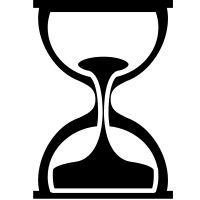
\includegraphics[height=.8em]{hourglass.png}}
\newcommand\hourglass{\usebox{\hourglassbox}}

%%%%%%%%%%%%%%%% SHORTCUTS FOR COMMONLY USED THINGS %%%%%%%%%%%%%%

\newcommand\Set{\textbf{Set}}
\newcommand\FinSet{\textbf{FinSet}}
\newcommand\MeasSet{\textbf{MeasSet}}
%\newcommand\MaxEnt{{\substack{\mathbf{Max}\\\mathbf{Ent}}}}
\newcommand\MaxEnt{{\overset{\uparrow}{\mathbf H}}}

%\def\bmu[#1|#2]{\boldsymbol\mu\boldsymbol{[} #1 \boldsymbol{|} #2 \boldsymbol{]}}

\newcommand\bb[1]{\mathbbm{#1}}

\newcommand\bmu{\boldsymbol{\mu}}
\newcommand{\V}{\mathcal V}
\newcommand{\N}{\mathcal N}
\newcommand{\Li}{\mathcal L}
%%%%%%%%%%%%%%%%%%%%%%%%%%%%%%%%%%%%%%%%%%%%%%%%%%%%%%%%%%%%%%%%%%



%%% What do I even call them anyway?
\newcommand{\ModelName}{Probabilistic Dependency Graph}
\newcommand{\modelname}{probabilistic dependency graph}
\newcommand{\modelnamehyper}{probabilistic dependency hypergraph}
\newcommand{\modelnames}{\modelname s}
\newcommand{\MN}{PDG}
\newcommand{\MNH}{PDH}
\newcommand{\MNs}{\MN s}
\def\seq{\!=\!}
\DeclareMathOperator\dcap{\mathop{\dot\cap}}

\title{\ModelName s}

\author{} % LEAVE BLANK FOR ORIGINAL SUBMISSION.

%% UAI  reviewing is double-blind.
%
%% The author names and affiliations should appear only in the accepted paper.
%%
%\author{
%	{\bf Oliver E. Richardson%\thanks{Footnote for author to give an alternate address.}
%		}\\
%%	Computer Science Dept. \\
%	Cornell University\\
%	Address\\
%\And
%	{\bf Joseph Y. Halpern}  \\
%	Cornell University      \\
%	Address \\
%}
%


\begin{document}
	\maketitle

	\begin{abstract}
		Graphical models cleverly compress probability distributions over joint settings of random variables, by making use of independence assumptions.
		
		However, because they model probability distributions, they are not expressive enough to represent mental states of agents who might not have globally consistent beliefs. 
			
		
%		We introduce \modelnames\ (\MNs) to combat these issues. \MNs\ are like unshackled Bayesian nets, interpreted more locally and whose links are interpreted as conditional sub-distributions. The result is a “graphical model” in a looser sense which may not always be either complete or consistent (from the perspective of a distribution), which can be easily combined with graph operations. We find that by solely altering the set of nodes and links and then running consistency reduction algorithm (one of which is a generalized version of belief propagation), we can recover important capabilities of Bayesian networks, such as the ability to estimate conditional and marginal distributions given observations, belief updating via Jeffrey’s rule. Further afield, we discover that this process also naturally models simple learning algorithms, and acting according to a decision rule (see the other paper for more). Bayesian networks, and to some extent, factor graphs, can be seen as special cases of \MNs.
	\end{abstract}

%	\tableofcontents

	\section{Introduction}
	% Want to resolve inconsistencies. can't talk abuot it until we can represent.
	% How to resolve (1) absent any information, or (2) I don't know, need further information.
	% inacurate to model people as having consistent 

	Inconsistencies are bad. Still, constantly examining every possible interaction between beliefs is taxing and restrictive, making inconsistency difficult to avoid: reasonable people are often simultaneously unaware of any inconsistencies in their beliefs, and yet still think it probable that they are not entirely consistent.%
		\footnote{In some sense, this is the reason arguments exist: it is possible to get a person to agree to premises and reject a conclusion, revealing inconsistency---inconsistency which can then be used to change someone else's mental state. }

		
	Most graphical models eliminate by fiat the possibility of inconsistency where possible, so that they can more naturally represent probability distributions, making them a poor tool for reasoning about inconsistent belief states
	While we do not endorse inconsistency, we nonetheless think it important to represent: in addition to modeling an overwhelmingly common feature of humans, the possibility of inconsistency 
	allows our model (called a \modelname\ or \MN)
	to portray intermediate stages of belief updating (\cref{sec:belief-update}), 
	provides a rationale for providing multiple justifications 
	(corroborating evidence means more in the presence of possible conflict; see \cref{ex:corrob}),
	and	recasts standard algorithms such as belief propagation and conditioning on evidence as resolutions of inconsistency (\cref{sec:algorithms}). 
	
	%While we share the distaste of inconsistency, we also see its possibility as an integral part of reasoning, and we will even be able to recover standard algorithms (conditioning, etc.) as special cases of inconsistency reduction (\cref{sec:algorithms}). 
		
%		\note{Part of the reason that it's hard to bring in modularity here is that the nature of the improvement differs depending on the model in question. Factor graphs arguably offer the same modularity---but there are other arguments against factor graphs that don't really bear on BNs}
	
	%%% ATTEMPT 1
	%As we will see, one reason these inconsistencies are difficult to avoid is our conceptual modularity: features of the world can be noticed, forgotten, and fragments of beliefs can be locally recombined long before they crystallize into global distributions or theorems.	
	
	%%% ATTEMPT 2
	%Separately, people enjoy conceptual modularity: features of the world (like the random variables which generate a graphical model) can be noticed, forgotten, and beliefs about their dependencies can be incorporated into our mental states without all of one's distantly unrelated beliefs.
	%These two features are in fact related, and we present here a representation of uncertainty which models both.
	
	The second feature of \MNs\ we wish to highlight is their modularity. We can leverage the new freedom to entirely remove the computational overhead and assumptions required to make structural changes to the graph (at the price of some inconsistency). 
	As a result, we can both make less conservative transformations of representation, and consolidate the computational costs of resolving them.
	
%	skirting computational costs and enabling concept formation, without also sacrificing interpretability, as factor graphs do (see \cref{sec:factor-graphs}). }
	The rest of this section consists of examples focusing on the benefits of possible inconsistency and improved modularity, and the failure of Bayesian Networks to capture what we have in mind (we later compare to other graphical models in \cref{sec:factor-graphs,sec:many-relations-graphical-models}). For a complete list of \MN\ features, and examples with the full formalism, see \cref{sec:list-of-benefits,}.
	
	\begin{example}\label{ex:guns-and-floomps}
		You arrive in a foreign country known for having very clear laws. From prior reading, you have subjective probability 0.95 that owning guns is against the law. Upon landing, you end up talking to some teenagers who use the local slang---after which you believe with 10\% probability that the law prohibits floomps.
		
		Let's try to represent this as a Bayesian Network. Make a graph with two nodes: let $F$ be the binary variable (taking values $\{f, \overline f\}$) indicating the legality of floomps, and $G$ (taking values $g, \overline g$) indicate the legality of guns. 
		The semantics of a Bayes Nets offer us two choices: assume that the two are independent, or choose a direction and make up some numbers for the table.
		As there is no reason to believe that either variable depends on the other, we opt for the latter, resulting the following ``network'':	
		
		\begin{center}
			\scalebox{0.9}{
			\begin{tikzpicture}[scale=0.8,ampersand replacement=\&]
	
				\node[dpadded, circle] (floomp) at (-1.2,0) {$F$};
				\node[dpadded, circle] (gun) at (1.2,0) {$G$};
	
				\matrix [table with head, column 1/.style={leftrule},
					 column 2/.style={rightrule}, row 2/.style={bottomrule}] at (-3.5,0)	{
					\vphantom{$\overline f$} $f$ \& $\overline f$\\
					.9 \& .1\\
				};
				\matrix [table with head, column 1/.style={leftrule},
					 column 2/.style={rightrule}, row 2/.style={bottomrule}] at(3.5,0)	{
					 \vphantom{$\overline g$}$g$ \& $\overline g$\\
					 .05 \& .95\\
				};
			\end{tikzpicture}
			}
		\end{center}
		
		You later discover that ``floomp'' is likely to be another word for gun, and come to believe that if floomps are legal (resp. illegal), then there's a 92\% chance guns are as well; let $E$ be the Conditional Probability Table (CPT) associated to this realization.
		A first reaction might be to simply add this conditional information by adding $F$ as a parent of $G$ and incorporating $E$ into the Bayes Net, but it is not clear what to do with our original CPT on $G$.
			% which amounts to throwing out our old prior distribution on $G$; 
			% another instinct might be to perform a Bayesian update, but this new information is conditional and probabilistic, not an event.
		In fact, $E$ conflicts with the other two tables, in the sense that there is no joint distribution on $\{F, G\}$ such that all three tables are accurate. 
		Therefore, there is no Bayes Net that contains all three pieces of information exactly: one has to resolve the inconsistency first.
			
			%There are three different dimensions along which this could be resolved: rejecting either prior belief, or $E$; in general any mixture would do. 
			
			
		Note that it may not be in your best interest to sort this out right away. The choice of resolution may be clearer if you can get confirmation that guns are indeed floomps, or read the laws more carefully---it may be worth sitting on the inconsistency so that you can resolve it properly later, rather than resolving it as best you can immediately.

%		\begin{enumerate} 
%			\item Even though the additional information takes the form of a conditional probability table, adding an edge with this table in our Bayes Net overwrites other information: by adding a link $F \to G$, the Bayes Net effectively overwrites our old beliefs about $G$. 
%%				By contrast, a Bayesian update cannot incorporate conditional information at all---only events.
%			
%			\label{item:noarrow}
%			
%			
%			\item It may not be in your best interest to sort this out right away. The choice of resolution may be clearer if you can get confirmation that guns are indeed floomps, or read the laws more carefully---it may be worth sitting on the inconsistency so that you can resolve it properly later, rather than resolving it as best you can immediately.%
%				\label{item:waiting-good}
%
%		\end{enumerate} 
		
		By contrast, consider the corresponding \MN,
		in which the CPTs are attached to edges, rather than nodes of the graph. 
		We will represent the CPT for a link $L \!\colon\! A\!\to\! B$ as matrices $\mat L$, whose element $\mat L_{a,b}$ at row $a$, column $b$ is the conditional probability $\Pr(B \!\!=\!\!b \mid A \!\!=\!\! a)$. 		
		In order to represent unconditional probabilities% (among other things; see section \ref{sec:algebra})
		, we introduce a \emph{unit variable}, $\mathsf 1$, or `$\mathrm{true}$', which always takes its unique value, $\star$. 
		
		\begin{figure}[h]
			\centering
			\scalebox{0.9}{
			\begin{tikzpicture}
				\node[dpadded] (true)  at (0,1.7) {$\mathsf 1$};
				\node[dpadded] (floomp) at (-1.5,0) {$F$};
				\node[dpadded] (gun) at (1.5,0) {$G$};			
				
				\draw[arr] (true) -- coordinate(A) (floomp);
				\draw[arr] (true) -- coordinate(B) (gun);
	
				\node[above left=0.5em of A] {
					\begin{idxmat}{$\star$}{$f$, $\overline f$}
						.90 & .10 \\
					\end{idxmat}
				};
				\node[above right=0.5em of B] {
					\begin{idxmat}{$\star$}{$g$, $\overline g$}
						.05 & .95 \\
					\end{idxmat}
				};
	
				\definecolor{heldout}{rgb}{0.7,0.7,1}	
				\draw[heldout, dashed, arr] (floomp) -- coordinate(C) (gun);
				\node[below=1em of C] {
					\color{heldout}
					E =\begin{idxmat}[\footnotesize\color{heldout}\text]{$f$,$\overline f$}{$g$, $\overline g$}
						0.92 & 0.08 \\ 0.08 & 0.92 \\
					\end{idxmat}
				};
			\end{tikzpicture}
			}
			\caption{An inconsistent \MN, requiring resolution}
			\label{fig:gun-floomp-diagram}
		\end{figure}
		
		The original state of knowledge consists of all three nodes and the two black edges from $\mathsf 1$. This is like our Bayes Net from before, except we no longer assume $F$ and $G$ to be independent% (but will later if necessary)
		---we merely record the constraints imposed by the given probabilities.
	
		\note{\emph{This is from our discussion but it seems out of the way of the story so I haven't integrated it.}
			A proponent of Bayes Nets would say: sure, we've assumed independence, but that was on purpose! We get a lot of mileage out of independence assumptions.
			
			If we wanted to explicitly encode such an independence assumption without making it part of the the background machinery for all diagrams, one would need to either give a link $F \to G$ (or vice versa) whose table has an identical distribution over $G$ every row, or specify the joint distribution directly, as below...
			
			\centerline{\scalebox{0.8}{
			\begin{tikzpicture}
				\node[dpadded] (true)  at (0,1.7) {$\mathsf 1$};
				\node[dpadded] (floomp) at (-1.5,0) {$F$};
				\node[dpadded] (gun) at (1.5,0) {$G$};
				\unmergearr{true}{floomp}{gun}
			\end{tikzpicture}
			}}
		
			These tricks save no representational space, making them useless for compressing distributions, and may not display the dependency structure you're looking for. We find 
			
			Using \MNs\ we can have our cake and eat it too:
		}
		
		$E$ can be added directly to the model as a link $F$ to $G$ without changing the meaning of the link from $\mathsf 1 \to G$, which we retain: the added modularity lets us simply include information, and resolve inconsistencies later. Unlike a Bayesian update, the operation is even reversible: all we need to do recover our original belief state is delete the new edge.

	\end{example}			
	
%	
%	\\Cref{ex:planet} highlights a difference \MNs\ }
%		
%		
%		, and also a third trait of interest: in addition to being so over-constrained as to be inconsistent with all distributions, \MNs\ can be too under-constrained to pick out a single distribution.
%	%		illustrate particularly well the biggest difference between the two interpretations of a graph: when two arrows point to the same node. 	
	
	The ability to represent these `over-constrained' states of belief, in which it is possible for there to be inconsistency, can also be valuable even when there is none. 
	Unlike other models, which require special coloring of nodes, \MNs\ also cleanly represent `under-constrained' beliefs, such as conditional ones, without modification.
	Our next example illustrates both, and highlights one more way in which BNs fail to be as modular as we might hope.
	
	
	\begin{example} \label{ex:planet}
		Suppose we have a belief about how size and composition affect the habitability of a planet: say we're astrobiologists, and we have some sense of how likely we are to find life on a given planet, supposing we knew its size (big or small) and its composition (mostly made of rocks vs gas), resulting in the CPT from \cref{fig:planet-initial}.
		
		\begin{figure}[h]
			\centering
			\scalebox{0.8}{
				\begin{tikzpicture}[center base]
				\node[dpadded,light pad,fill opacity=.2] (SS) at (0.2, 1.2) {Size};
				\node[dpadded,light pad,fill opacity=.2] (CC) at (2.6, 1.2) {Composition};
				\node[dpadded,light pad,fill opacity=0] (LL) at (1.4,0) {Life};
				\node[dpadded,light pad,fill opacity=.1, dashed, text opacity=0.3] (WW) at (-0.5, 0) {Water};
				\draw[arr] (CC) -- (LL);
				\draw[arr] (SS) -- (LL);
				\draw[arr, dotted, opacity=0.5] (WW) -- (LL);
				\end{tikzpicture}	
			}%		
			~~\scalebox{0.8}{
%			$\Pr(\text{Life} ~|~ \text{Size}, \text{Comp}) =$\\
			$\begin{idxmat}{{big, rocks}, {small,rocks}, {big, gas}, {small,gas}}{life, no life}
				.1 & .9 \\
				.2 & .8 \\
				.05 & 0.95 \\
				0.001 & 0.999
			\end{idxmat} $}
			\caption{CPT and desired new node in \cref{ex:planet}}
			\label{fig:planet-initial}
		\end{figure}
		\vspace{1em}
	
		Ignoring the faint ``water'' node for now, the diagram on the left corresponds to the \emph{conditional} Bays Net on the left---note that the nodes `Size' and `Composition' would need tables of their own to be fully interpreted as a Bayesian Network. Without any such beliefs, we would have to use a \emph{conditional} Bayes Net, and explicitly mark both nodes as `observed'.
		
		\begin{vfull}
			A proponent of BNs will have no trouble getting this to work by using \emph{conditional} BNs, which represent conditional distributions rather than joint ones, with two slight inconveniences: (1) they would have to commit which variables are conditioned up-front, and so adding or removing information changes the type of mathematical object represented, and (2) there is no graphical distinction between having a distribution over $\sf Size$ or not, and so we have to color certain nodes and keep track of this additional information. \MNs\ have neither of these issues, but the bigger payoff is in representing \textit{over-constrained} states.
		\end{vfull}

		Now our biologist friend now reminds us that life requires water, and computes probabilities for the existence of life on a planet, with and without water. We trust this friend completely. We'd like to introduce a new node, `Water', but if we make it a parent of `Life', because we don't know how this information interacts with size, and composition; neither are we prepared to give a probability of live given a full description of the three, and this table would be much larger.%
			\footnote{If \textit{Size} and \textit{Composition} each had $\approx\sqrt{N}$ elements, and \textit{Water} had $\approx N$ elements, it would be $O(N^2)$ to store a full joint table, compared to $O(N)$ for the two individual ones.} %At this point the Bayesian Network is not at all a convenient way of storing the information at hand.
		Let $S, C, W, L$ be the respective shortenings of our variables.
		\MNs\ allow us to interpret the last arrow individually, using a picture like this:

		\begin{center}
		\scalebox{0.9}{
		\begin{tikzpicture}
			\node[dpadded] (S) at (0.2, 1.4) {$S$};
			\node[dpadded] (C) at (2.4, 1.4) {$C$};
			\node[dpadded] (L) at (1.3,0) {$L$};
			\node[dpadded] (W) at (-1,0) {$W$};
			\cmergearr{S}{C}{L}{1.3,0.95}
			\draw[arr] (W) -- (L);
		\end{tikzpicture}}
		\end{center}
	
		This means that we have two conditional probability tables on $L$: one from $S \times C$ and the other from $W$. We can now combine our two beliefs, without also providing information about the correlations between $W$ and $S\times C$ we do not have. As with the previous example, there is now a possibility of being inconsistent, in the sense that is possible to specify the conditional distributions in the links in such a way that no joint distribution on all variables will marginalize out to them --- for instance, if all estimates of $L$ from the $W$ are strictly smaller than any probability estimate of $L$ from $S \times C$.
	\end{example}
	
%	Though perhaps difficult to see in example \Cref{ex:guns-and-floomps},
	\MNs\ are strictly more expressive than Bayesian Networks, and there is a straightforward conversion from a BN to a \MN\ (section \ref{sec:bn-convert}). 
	%The two graphical models also look alike (and indeed are exactly the same for linear chains of variables);
%	\note{Changed. The focus was wrong in the previous one you told me to cut, but this part is still useful I think.} 
	In some sense, the biggest difference between \MNs\ and BNs is the interpretation of two colliding arrows, as highlighted in \cref{ex:smoking}.
	
	

	\begin{example}\label{ex:smoking}
		Consider the classic example used to introduce Bayesian nets, in which the four variables are interest are booleans indicating whether a person ($C$) develops cancer, ($S$) smokes, ($SH$) is exposed to second hand smoke, and ($PS$) has parents who smoke, presented graphically in \cref{subfig:smoking-bn}.
		\begin{figure*}[ht!]
			\centering
			
			\begin{subfigure}[b]{0.3\textwidth}
				\scalebox{0.9}{
				\begin{tikzcd}[center base, column sep=1.8em, row sep=1em, dpad={fill opacity=0, draw=gray}, 
					ampersand replacement=\&]
				\& S \ar[dr] \\
				PS \ar[ur]\ar[dr] \&\& C \\
				\& SH \ar[ur]
				\end{tikzcd}}
				\caption{Bayesian Network}
				\label{subfig:smoking-bn}
			\end{subfigure}%			
			\hspace{2em}\vline\hspace{2em}
			\begin{subfigure}[b]{0.5\textwidth}
				\scalebox{0.9}{
				\begin{tikzpicture}[center base]
				\node[dpadded] (1) at (0,0) {$\mathsf 1$};
				\node[dpadded] (PS) at (1.65,0) {$PS$};
				\node[dpadded, fill opacity=0.16] (S) at (3.3, 0.8) {$S$};
				\node[dpadded, fill opacity=0.16] (SH) at (3.3, -0.8) {$SH$};
				\node[dpadded, fill opacity=0.16] (C) at (4.8,0) {$C$};
				
				\draw[arr] (1) -- (PS);
				\draw[arr] (PS) -- (S);
				\draw[arr] (PS) -- (SH);
				\mergearr{SH}{S}{C}
				
				\node[dpadded, fill opacity=0.05,dashed] (T) at (6.5,0) {$T$};
				\draw[arr,dashed] (T) -- (C);	
				\end{tikzpicture}}
				\caption{Corresponding \MN}
				\label{subfig:smoking-pdg}
			\end{subfigure}
		
			\caption{Both graphical models representing the conditional relationships in \cref{ex:smoking}}
			\label{fig:smoking-bn+pdg}
		\end{figure*}
		
		The BN is a compact representation of a joint distribution over all four variables, which achieves compactness by taking advantage of independence between variables. It encodes an assumption that every node is independent of its non-descendants given its parents.
		Most of the time, we do not make the independence assumption because we know for certain that the variables are independent; rather, we just suspect that the identified links are by much more important than the others. Determining for sure that smoking  and second hand smoke are independent, controlling for parents' smoking habits, would extremely difficult, and would require empiricism to validate.
		
		The \MN, on the other hand, represents merely the set of constraints on marginals given in the tables. Depending on our chosen semantics (we offer several in section \ref{sec:formal+semantics}), we can further interpret the constraints. For instance, by looking at the maximum entropy distribution consistent with the constraints, we get back the independence assumptions from the BN, and can thereby view \Cref{subfig:smoking-pdg} as representing the same distribution as the BN.
				
		Now, suppose you read a very thorough empirical study which demonstrates that people who use tanning beds have a 10\% incidence of cancer, compared with 1\% in the control. Just as in the previous example, this cannot be encoded directly into the Bayesian Network. 
		The \MN\, on the other hand, has no trouble, and is simply the union of the two pieces of information, as in \ref{subfig:smoking-pdg}.
		
%		\begin{center}
%			\scalebox{0.9}{
%			\begin{tikzpicture}
%			\node[dpadded] (1) at (0,0) {$\mathsf 1$};
%			\node[dpadded] (PS) at (1.65,0) {$PS$};
%			\node[dpadded, fill opacity=0.16] (S) at (3.3, 0.8) {$S$};
%			\node[dpadded, fill opacity=0.16] (SH) at (3.3, -0.8) {$SH$};
%			\node[dpadded, fill opacity=0.16] (C) at (4.8,0) {$C$};
%			\node[dpadded, fill opacity=0.05,dashed] (T) at (6.5,0) {$T$};
%			
%			\draw[arr] (1) -- (PS);
%			\draw[arr] (PS) -- (S);
%			\draw[arr] (PS) -- (SH);
%			\mergearr{SH}{S}{C}
%			\draw[arr,dashed] (T) -- (C);
%			\end{tikzpicture}}
%		\end{center}
		
		As before, simply adding $T$ to the parents of $C$ makes it impossible to use the old table, and require us to guess at the interactions between tanning beds and smoking.
		% This is again an illustration of the modularity and the possibility for inconsistency; compare the right half of the diagram (shaded slightly darker) with the topological equivalent in example \ref{ex:planet}.
	\end{example}	


	%\todo{One final example, this time with directed factor graphs? Or illustrate power of sub-stochasticity?}
	
	
	For our final introductory example, we will show how we can use the modularity and this interpretation of arrows to do more complicated reasoning.

	% Worry: this example may be too first-order, and I might not understand the 
	% connections to first order logic well-enough to put them in the UAI paper.
		% But: It does help explain why sub-stochasticity is natural. I'm not really relying on it being full FoL; it might be expressible with modalities and is probably much weaker still
	\begin{example}
		You're a math teacher. You used to teach at $A$, which is in a poorer area and rated more poorly, and now teach at $B$, where the students care more about education. The institutions both teach differential equations, but in different ways: $A$ focuses on numerics, whereas $B$ focuses on analytic solutions.
		
		You you're about to give a test on Laplace transforms.
		You have some distribution $G_B$ of likely grades for students in $B$, but you also have a good model of the distribution $G_A$ of grades a student from $A$ might get. We want to model this epistemic state, and now present three alternative modeling choices.

		Here are three alternative modeling choices: we can either (1) use a single variable $\cal I$ whose values are possible institutions, (2) have separate variables for each institution, or (3) have different variables for grades of students.
		
		\begin{center}
			\todo{diagram of (1) and (2)}
%			\begin{tikzpicture}
%				\node[dpadded] (I) at (0,0) {$I$};	
%				\node[dpadded] (L) at (0,2) {$\mathcal L$};
%			\end{tikzpicture}
		\end{center}
		
		If you do (1), and want to express $G_A$ and $G_B$ as a link $\mathcal  I \to G$, where $G$ is the resulting grade, then you must also supply a distribution on $G$ for every other institution you think a person could be from. $\mathsf {Inst}$ cannot only take values $\{A,B\} $, because obviously you know of other schools, but you may not have a good sense of what they do, nor even what kinds of students they attract. 
			Note that this would be ok for modeling a game where we first select an institution from $\{A, B\}$, and then a grade from some true underlying distribution. We would also have been ok modeling the situation in which $\cal I$ were used as the target of another link, like which institution a given student were looking over --- 
		
		We can try to get around this by letting $\mathcal  I$ take values $A$, $B$, and ``other'', but now you need to supply a distribution on grade given ``other''; maybe this is just like an unconditional distribution on grades. You might not know whether which school is more ``average'' nor even what the appropriate reference frame is: do you take an average by state, or country? And how much do you need to correct your estimate given that ``other'' does NOT include $A$ or $B$? This is implausible to estimate. 		
	
		%TODO (2): using indicator variables
		
		%TODO (3): using two G vars
		
		Ultimately the problem is a lack of expressive power and modularity: we need a way of letting 
		

		
		
		
%		You really have no idea how well a student would do from other institutions would do, as you're not familiar with their material or the kind of people they attract. 
		

	\end{example}

	While other graphical representations (such as factor graphs) are also more modular, they do not represent inconsistency either, and raise their own issues (see \cref{sec:factor-graphs}). 
	
	Thus far, we have given a taste of why \MNs\ could be valuable: they can represent under and over-constrained epistemic states, allow us to avoid making unnecessary assumptions, and are more modular, in the sense that changes to the underlying graph are much simpler and require fewer assumptions than for Bayesian Networks.	
	%
	%However, we have only described parts of our simplest model; before we get to the more powerful variants, we need to formalize what we have.
	
	
	

%	\begin{enumerate}[nosep]
%		\item This representation more naturally matches what humans are aware of, encoding small locally consistent models rather than one giant probability distribution
%		\item It is a strictly more general representation--- we can easily convert BNs to these diagrams (section \ref{sec:convert2bn})
%		\item This allows composition of arrows to be defined, and gives meanings to paths (section \ref{sec:composition}).
%		\item Allowing variables to be added and removed makes
%		\item Changing and partially determining arrows is more reasonable.
%		\item We can now represent inconsistency, which will allow us to capture mental states which, and . While we agree with the classical picture in that inconsistency is bad, now we can talk about it
%	\end{enumerate}


	% Redundency is important: types in programming languages, more data in ML systems.
	% Puts gurads
	% Makes it possible to combine knowledge without destroying old knowledge.
	% preference updating
	
	
	\section{Formal Definitions and Semantics}\label{sec:formal+semantics}
	
%	We give the definition below for the finite case.  
	
	We have seen some examples of \MNs, but elided the details; we now begin a more careful treatment of \MNs\ as mathematical objects. Rather than representing a probability distribution, \MNs\ can be thought of as (soft) \emph{constraints} on distributions.

	
	
	Compared to a Bayseian Network, a \MN\ still consists of a directed graph, and the edges still inform conditional probability tables, but now each edge is interpreted individually. For instance, the node $C$ in the graph
	\[ A \!\rightarrow\! C \!\leftarrow\! B,\]
	which would be interpreted as a single table $\Pr(C\mid A, B)$ in a BN, would be two separate tables $\Pr(C \mid A)$ and $\Pr(B \mid A)$ in a \MN. We now give two definitions of \MNs\, which will turn out to be equivalent by \cref{thm:hyperequiv}.

	%
	
	\def\mnvars[#1]{(\mathcal N#1, \mathcal L#1, \mathcal V#1, \bmu#1)}
	\begin{defn}[\MNH]\label{def:hypermodel}
		A \emph{\modelnamehyper} is a tuple $\mnvars[]$ where
		\begin{itemize}[nosep]
			\item $\N$~~is a finite collection of nodes
			\item $\Li \subseteq 2^{\N} \times 2^{\N} \times \mathrm{Label}$~~is a set of directed links, each of which has a source and target subset of $\N$.
			\item $\V$ associates each node $N \in \mathcal N$ with a set $\V(N)$ or $\V_N$, representing the values that node $N$ can take.
			\item $\bmu$
			 % $\colon\!\big(\!({\bf A,B})\colon \! \Li \big) \to \prod\limits_{A\in \bf A} \!\! \V(A) \to \underline\Delta\left[\prod\limits_{B \in \bf B}\!\!\V(B)\right]$
			%%% Above is the type of $\bmu$. I think it's important to have it there.
			associates conditional probability (sub)-distributions on the joint settings of $\bf B$ indexed by the joint settings of variables in $\bf A$ for every link $({\bf A,B}) \in \mathcal L$ %
		\end{itemize}

	\end{defn}

	These characterize will often use two additional bits of syntax: $\sf 1$ is a variable that can only take one value.
	
	\todo{}

	The name is chosen because each arrow is a conditional pseudo-marginal, in that they might not
	globally be the marginals of a single distribution, but they are all locally consistent. 
	%	\begin{defn}
	Here $\underline\Delta(X)$ is the collection of sub-distributions on $X$ --- i.e., distributions on $X \cup \{*\}$, where $\{*\}$ is a `null' element. 

	\begin{defn}[\MN]\label{def:model}
		A \textit{\modelname} is a \modelnamehyper\ where every link has just one source and target node.
	\end{defn}

	We will call a \MN/\MNH\ \emph{strict} if $\bmu$ assigns no mass to $\bullet$. The examples we have seen thus far are strict, but we explore the implications carefully in section \ref{sec:full-model}.

	
%	\end{defn}
	




	


%	If every $\mathcal V(N)$ is finite with all subsets measurable, then $\bmu_{A,B}$ is just a conditional probability table, or a stochastic matrix.
%	You may have noted that this only includes data for the normal arrows, rather than the multi-tailed ones described in the examples. This can be achieved either by generalizing $\mathcal L$ to higher orders, or introducing product nodes; we opt for the latter as it simplifies the formalism and paves the way for additional special nodes in \cref{sec:algebra}.

	

	\begin{vfull}
		This works pretty well for the two edges that we described before, but the structural overhead of the additional de-sugaring: the $\boldsymbol\mu[S\times C\to S]$ and $\boldsymbol\mu[S\times C\to C]$ tables, as well as the set $\mathcal V(S \times C)$ seem like they didn't need to be specified, and one might even feel that it would be a mistake to allow any other table. Some reasons for this design decision include:
		\begin{itemize}[nosep]
			\item It is easier to prove things about graphs than directed hyper-graphs. Similarly, defining composition and paths becomes a lot simpler.s
			\item We can eliminate the clunkiness by fusing the model with an algebra, as in \cref{sec:algebra} --- which will give us a lot more than modeling the hyper-edges directly.
			\item We will eventually also want to allow for the possibility of keeping only a relaxed, approximate representation of $\mathcal V$ and $\bmu$, and in particular, of the ones constructed logically in this way. By specifying them explicitly for now, we will have to do less work to regain manual control in \cref{sec:abstraction}
		\end{itemize}
	\end{vfull}


	Now some notation: If $M = \mnvars[]$, let 
	$$W_{\cal V} \seq W_M :=  \prod_{N \in \mathcal N}\mathcal V(N),~~ W_{\cal V}^\bullet = \prod_{N \in \mathcal N}\Big(\mathcal V(N) \cup \{\bullet\} \Big)$$
			
%	\section{Semantics}\label{sec:semantics}
	These graphs admit multiple semantics. We think of \modelnames\ as being a representation of beliefs in and of themselves, rather than a compression of something more fundamental such as a probability distribution. Still, we will find it useful to interpret them in various ways: doing so will make it possible to compare them more directly with existing graphical models, which one thinks of as really just being compressed distributions. In this section, we would like to highlight three important semantics.
	
	\subsection{As Sets of Distributions}\label{sec:set-of-distribution-semantics}
	If the focus is on under-constrained models, then just as a BN represents a distribution on joint space, a \MN\ might be thought of as representing the set of all distributions that marginalize out to it exactly. 
	
	
	\begin{defn}
		Let $M \!=\!\mnvars[]$ and $M'= \mnvars[']$ be \MNs\ with \todo{I forget where this was going}
	\end{defn}
	

	
	\begin{defn}
		If $M\seq\mnvars[]$ is a \MN, let $\llbracket M \rrbracket_\Set$ be the set of distributions over the variables in $M$ consistent with $\boldsymbol\mu$ on every pseudomarginal. Formally,		
		\[ \Big\llbracket M \Big\rrbracket_\Set \hspace{-2ex} := \!\left\{\mu \!\in\! \Delta W_{\cal V}^\bullet\ \middle|\!
		\begin{array}{l}
		\mu(B\!\! =\!\!b \mid A\!\!=\!\!a) \geq \boldsymbol\mu_L(b \mid a) \\[0.1em]
		~\text{$\forall (A, B, L) \!\in\! \mathcal L$, $a \!\in\!\mathcal V_A$, $b \!\in\! \mathcal V_B$} \end{array}\!\!\! \right\}\]
	\end{defn}
	
	
	Notice that $S := \bbr{
		A \overset{p}{\to} B
	}_\Set$ has a natural identification with 
	the conditional distribution $p( B \mid A)$. $S(b\mid a)$ is well-defined since $\mu(\cdot\mid a)$ is the same for all $\mu \in S$ (and unique since it's the only commonality). Both features are normally achieved in a less flexible manner: by coloring nodes and explicitly separating out the ``observed'' nodes at the beginning of the construction.
	We can also now finally give a formal definition of consistency.
	\begin{defn} \label{def:weak-consistent}
		$M$ is consistent if there is some $\mu \neq \mu_\bullet \in \bbr{M}_\Set$, and strictly consistent if there is some $\mu \in \bbr{M}_\Set$ that assigns no mass to a world where any variable takes $\bullet$.
	\end{defn}
%	The `weakly' can be omitted; we introduce it here to contrast it with a stronger version in \cref{def:strong-consistent}.
	
%	Sometimes, not all of the a-priori worlds will actually be possible: some may be in logical contradiction with one another, such as if $A \times B$ takes the value $(a,b)$ and $A$ takes $a' \neq a$.
%	\begin{defn}
%		Consider again the \MN\ $M = (\mathcal N, \mathcal L, \mathcal V, \bmu)$. Define 
%		\[ W_M := \{ w \in W_{\cal V} : \mu(w) > 0 \text{ for some } \mu \in \bbr{M}_\Set \} \]
%	\end{defn}
	
	If $R$ and $S$ are sets of distributions, $R$ over the variables $\mathbf X$ and $S$ over $\mathbf Y$, then
	$$R \dcap S := \{ \mu \in  \Delta \mathcal V(\mathbf X \cup \mathbf Y) : \mu_{\mathbf X}, \mu_{\mathbf Y} \in R \times S \}  $$
	\begin{prop}
		$\bbr{M}_\Set \dcap \bbr{M'}_\Set = \bbr{M \cup M'}_\Set$.
	\end{prop}

	
	
	\begin{lemma}[restate=thmsetconvex] 
		\label{prop:convex}
		$\bbr{M}_\Set$ is convex, for any \MN\ $M$.
	\end{lemma}%


%	\begin{conj}
%		If $\mathcal P$ is a closed, recursive, convex set of probability measures, then there is a \MN\ $M$ such that $\bbr{M}_\Set = \mathcal P$ 
%	\end{conj}




	\subsection{As Weighted Distributions}
	
	
%	If a probability distribution is a soft constraint on the set of possible worlds, then a \MN\ is a soft constraint on the set of probability distributions.
	
	In specifying a distribution via a graphical model, you have not only implicitly defined not only the distribution you intended, but also a natural higher-order scoring on distributions not only through the description of the distribution 
	
 	This generalizes the semantics in the previous section. For a candidate distribution $\mu$, rather than assigning it a 0/1 score of whether or not it is consistent, we give it a continuous one.

	\begin{defn}
		The inconsistency, $\zeta$, of a \MN\ $M = (\cal N, L, V, \bmu)$ with respect to a distribution $p \in \Delta[W_{\cal V}]$ is
		\[
			\zeta(M ; p) := %\inf_{p \in \Delta(W^{\mathcal V})}~
			\sum_{L \in \cal L}~\mathop{\mathbb E}_{a \sim p(A)} \left[\kldiv[\Big]{\bmu_{L}(a) }{ p(B \mid A = a) } \right]
		\]
		where $D_{KL}$ is the relative entropy, taken between the two distributions over $B$: one given by the link from $\bmu_{A,B}(a)$ and the other given by the marginal distribution of $p$ conditioned on $A = a$, over the variable $B$.
	\end{defn}	
	
	If we think of the inconsistency as a potential energy, we can use something like a Boltzmann law to get likelihood over distributions. We therefore define	
	\[\bbr{M}_\zeta := \mu \mapsto e^{-\zeta(M;\mu)}\]


	\begin{prop}[restate=thmzetaconvex]
		$\zeta$ is a convex function in $p$.
	\end{prop}
	As a result, $\bbr{M}_\zeta$ is a quasiconvex function, and hence local optimization will find global optima.

	\begin{defn}
		The inconsistency of a \MN\ $M = (\cal N, L, V, \bmu)$ is the minimum value that could be achieved with any test distribution $p$; that is, 
		\[ \zeta(M) = \inf_{ \mu \in \Delta [W_{\cal V}]} \zeta (M; \mu) 
%			= -\log \sup_{p \in \Delta[W_{\cal V}]} \bbr{M}_\zeta (p)
			 \]
		
	\end{defn}


	We may also consider the links as having different strengths: if we associate a positive `inverse temperature' coefficient $\beta$ to each edge.
	
	\begin{defn}
		A weighted \MN\ $(M, \beta)$ is a \MN\ $M = (\cal N, L, V, \bmu)$ together with an inverse temperature $\beta_L \in \mathbb R^+ \cup \{\infty\}$ for each link $L \in \mathcal L$.
	\end{defn}

	We an always take a \MN\ $M$ and uniformly assign every edge the same inverse temperature $\beta$; we'll call this $M^{-\beta-}$.
	
	\begin{prop}
		If $M$ is consistent, $\bbr{M^{(\infty)}}^* = \bbr{M}_\MaxEnt$.
	\end{prop}


	\begin{example}[continues=ex:guns-and-floomps]
		Recall the \MN\ from our first example, in figure \ref{fig:gun-floomp-diagram}. Suppose that both the of the initial links $1 \to F$ and $1\to G$ have temperature 1, and we give our new observation $10^{-3}$.
		
		Then $\bbr{M}_\zeta$
		\todo{}
	\end{example}	
	
	
	
	
	\subsection{As Distributions}
	
%	\[ \Big\llbracket M \Big\rrbracket^{\ell}(\mu) := \left\{\mu \in \Delta\left[~\prod_{N \in \mathcal N}\mathcal V(N)\right] ~\middle|~
%	\begin{array}{l}
%	\ell(\mu) \succeq \ell(\mu') \\[0.2em]
%	\qquad\text{for all $\mu' \in \Delta \prod \mathcal V$} \end{array} \right\}\]
	
	When ultimately pressed on a decision, an agent hasincentives to temporarily act as though their beliefs were simply a distribution. Via maximum-entropy semantics, we also offer a way of interpreting a \MN\ as a single distribution for this purpose. 
	
	\begin{defn}
		If  $M$ is a \MN, $\bbr{M}_{\mathbf S} \subseteq \Delta W_{M}$ is a set of distributions, $(D, \preceq)$ is an ordered set, and $\ell : \Delta W_{M} \to \mathbb (D, \leq)$ is a scoring function for probabilities, let \emph{the upper $\leq$-frontier under $\ell$}, denoted $\bbr{M}_{\mathbf S}^\ell$, be the set of distributions that are not strictly dominated by any others. Explicitly,
%% ALTERNATE, BIG
%		\[ \Big\llbracket M \Big\rrbracket^{\ell}(\mu) := \left\{\mu \in \Delta\left[~\prod_{N \in \mathcal N}\mathcal V(N)\right] ~\middle|~
%			\begin{array}{l}
%			\ell(\mu) \succeq \ell(\mu') \\[0.2em]
%			\qquad\text{for all $\mu' \in \Delta \prod \mathcal V$} \end{array} \right\}\]
		\begin{align*}
			\llbracket M \rrbracket_{\mathbf S}^\ell &=  \left\{\mu \in \llbracket M \rrbracket_{\mathbf S} ~\Big|~ \forall \mu' \in \llbracket M \rrbracket_{\mathbf S}.~ \ell(\mu') \preceq \ell(\mu)  \right\} \\
%			\llbracket M \rrbracket^{\bf S}_\ell &= \left\{\mu \in \llbracket M \rrbracket_\Set ~\Big|~ \forall \mu' \in \llbracket M \rrbracket_\Set.~ \ell(\mu) \geq \ell(\mu')  \right\} 
		\end{align*}
	\end{defn}
	One particularly useful scoring function is the following one, maximizing Shannon entropy:
	\[ \Big\llbracket M \Big\rrbracket_\MaxEnt := \Big\llbracket M \Big\rrbracket_\Set^{-H(\cdot)} \]

	\begin{theorem} 
		If $M$ is consistent, then $\bbr{M}_\MaxEnt$ contains a unique distribution; otherwise $\bbr{M}_\MaxEnt$ is empty.
	\end{theorem}
	\begin{proof}
		\vspace{-1em}
		This is a direct consequence of \cref{prop:convex}
	\end{proof}


	
	
	Now that we have all stated all three formal semantics of $\MNs$

	
	

	\begin{theorem}[restate=thmhyperequiv]\label{thm:hyperequiv}
		Every \modelnamehyper\ $M$ is equivalent to a \MN\ $M'$ with additional variables. That is, for each semantics $\bbr{-}$ and transformation $\varphi$ we define, $\bbr{M} = \bbr{M'}$ and $\varphi(M) = \varphi(M')$.
		%		\todo{define ``equivalence'' and prove.}
	\end{theorem}
	\begin{proof}
		This is done by introducing a new node corresponding to every non-singleton set of variables that participates in a link. For instance, the \MN\ in \cref{ex:planet} is translated as follows:
		\begin{center}
			\scalebox{0.8}{
				\begin{tikzpicture}
				\node[dpadded] (L) at (1.3,0) {$L$};
				\node[dpadded] (W) at (-0.5,0) {$W$};
				
				\node[dpadded,light pad, dashed] (SC) at (3, 0){\footnotesize $S \times C$};
				\node[dpadded] (S) at (5, 0.5) {$S$};
				\node[dpadded] (C) at (5, -0.5) {$C$};
				
				\draw[arr, ->>] (SC) -- (S);
				\draw[arr, ->>] (SC) -- (C);
				\draw[arr] (SC) -- (L);
				\draw[arr] (W) -- (L);
				\end{tikzpicture}}
		\end{center}
		See \cref{sec:hyper-convert} for the full example and proof.
	\end{proof}
	
	This theorem allows us to consider any \MN\ as merely an ordinary collection of nodes and edges, which rely on to define and compose paths.
	

	
%	This corresponds to a lexicographical ordering on \emph{all} distributions (as opposed to simply the ones in $\bbr{M}_\Set$), where we order first by satisfaction of constraints, and then by entropy. In general, we might be willing to relax the constraints a little, and sacrifice some fit for aa more general distribution. This allows us to define a free energy; see \cref{sec:thermo} for more.
	
	\subsection{As Probabilisitic Programs}\label{sec:prog-semantics}
	
	Conditional distributions can be thought of as probabilistic programs. As a result, we can compose and run them --- one  benefit to keeping local data in the form of conditional distributions is that you can compose them; paths from $A$ to $B$ correspond to noisy estimates of $B$ from $A$.
	
	Specifically, if $f(b \mid a) : \mathcal V_A \to \Delta \mathcal V_B$ and $g(c \mid b) : \mathcal V_B \to \Delta \mathcal V_C$ are conditional distributions, then the probabalistic composition $g\circ f : \mathcal V_A \to \Delta\mathcal V_C$ is
	\begin{align*}
			(g\circ  f) (c \mid a) :=  \sum_{b \in \mathcal V B}\!\! f (b \mid a)\ g(c \mid b)
	\end{align*}
	
	This can be recognized as a matrix multiplication $f$ and $g$ regarded as sub-stochastic matrices.
	Thinking about grpahical models this way makes thinking about chains of reasoning simpler, gives us a way out of storing probability tables, and suggests additional applications.
	% It also has not escaped us that \MNs\ have a particularly nice description in categorical terms, which we do not pursue further here.
	
	Furthermore, thinking about the mental state of an agent as a collection of programs you could run from any concept gives our first interpretation of a sub-distribution: probability mass assigned to $\bullet$ by a link $p$ has not terminated yet (if at all). 
	
	\begin{defn}
		A \MN\ $M$ is \emph{strongly consistent} if every collection of paths $\{P_i\}_i$ is compatible, in that 
		$$\bigcap_i\ \bbr*{\vphantom{\Big|}p_i^0\circ \cdots\circ p_i^k}_\Set \neq \varnothing$$
	\end{defn}

	\begin{prop}
%		$ \text{strongly consistent}  \subsetneq \quad 
%		\text{strictly consistent}  \subsetneq  \text{consistent} $
		Any \MN\ $M$ that is strongly consistent is also consistent, but some strongly consistent \MNs\ are not strictly consistent.
	\end{prop}

%	\begin{example}
%		The trace graph of a 
%	\end{example}
	
	
	% This means we can sample them
	% Also, compose them
	% and a

	\section{Relations to Other Graphical Models}\label{sec:other-graphical-models}
	
	Bayesian Networks may be the most widespread graphical models, but they are certainly not the only ones. In some sense, each can emulate the others, to various degrees of ease. A large number of them can be seen in \cref{fig:model-transformations}. Here we will only a few of the most important classes; see \cref{sec:many-relations-graphical-models} for more.

	\usetikzlibrary{decorations.markings}	
	\begin{figure*}[t]
		\centering
		\begin{tikzpicture}
			\begin{scope}[every node/.style={ellipse, fill, fill opacity=0.05,text opacity=1,
						outer sep=3pt,font=\bfseries}, xscale=2.5,yscale=1.2]
				\node (KB) at (-3, 0.5) {KB};
				\node (CG) at (-3, 1.5) {CG};

				\node (CRF) at (-1.2, 0.4) {CRF}; % CFG
%				\node (CRF) at (-2, 0) {CRF};
			
				\node (MRF) at (-2, 1) {MRF};
				\node (FG) at (-1,1.35) {FG};
				\node (SDFG) at (0,1.5) {FG$^\rightharpoonup$};
				\node (DFG) at (1,1.35) {FG$^\rightarrow$};
				\node (BN) at (2,1) {BN};

				\node (CBN) at (2,0) {CBN};
				\node (DN) at (1.3, 0.6) {DN}; 

				\node (sPDGH) at (0,0.5) {sPDG$_{\text{hyper}}\!\!$};
				\node (PDGH) at (-0.8,-.5) {PDG$_{\text{hyper}}\!\!\!$};
				\node (PDG) at (0,-.85) {PDG};
				\node (sPDG) at (0.8,-.5) {sPDG};

				\node (prog) at (3, -0.2) {PProgSet};
				
				\node (CPS) at (1, -1.4) {CPS};	
				\node (PlateBN) at (-2.5, -1.2) {PlateBN};
				\node (LPS) at (-1,-1.4) {$\underline {\mathcal P}$};
			\end{scope}
	
			% lossless		
			\begin{scope}[every edge/.append style={->}]%right hook->
				\draw (BN) edge (DFG) (DFG) edge (SDFG);
				\draw (MRF) edge (FG) (FG) edge (SDFG);
%				\draw[->] (DFG) -- (FG);
				\draw (CBN) edge[bend left = 5, shorten >=7pt] (sPDGH);
				\draw (CG) edge[bend left=10] (FG);
				\draw (KB) edge (CG);
				
				\draw (sPDGH) edge (PDGH) (sPDG) edge (PDG);
				
				\draw (BN) edge (DN) (DN) edge (sPDGH);
				\draw (DFG) edge (sPDGH);
				
				\draw (MRF) edge (CRF);% (CRF) edge (CFG);
				\draw (BN) edge (CBN);
				\draw (FG) edge (CRF); %crf
				
				\draw (CG) edge[out=-55, in=195, looseness=1.5, shorten >=7pt] (sPDGH);
				\draw (prog) edge[bend left=5] (sPDG);
				\draw (CPS) edge[out=180,in=-30] (PDG);
				\draw (PlateBN) edge[bend right=5] (PDGH);
				\draw (LPS) edge[out=0, in=-150] (PDG);
			\end{scope}
	
			% PDG Equivalences
%			\draw[->, transform canvas={yshift=2pt}] (PDGH) -- (PDG);
%			\draw[->, transform canvas={yshift=-2pt}] (PDG) -- (PDGH);
%			
%			\draw[->, transform canvas={yshift=2pt}] (sPDGH) -- (sPDG);
%			\draw[->, transform canvas={yshift=-2pt}] (sPDG) -- (sPDGH);
			
			\draw[double equal sign distance, shorten <=0pt, shorten >=0pt] (PDGH) -- (PDG);
			\draw[double equal sign distance] (sPDGH) -- (sPDG);

			
			% Projections. Lose information but preserve something.
			\begin{scope}[every edge/.append style={densely dashed, red, ->}]
				\draw (sPDGH) edge[bend left=10, out=10] (FG) (sPDGH) edge[bend right=10, out=-5] (FG);
				\draw (SDFG) edge[bend right=20] (FG);
			\end{scope}
			% Inefficient conversions.
			\begin{scope}[every edge/.append style={ultra thick, dotted, line cap=round, shorten >=2pt,
					decoration={markings,mark=at position 1 with {\arrow[xshift=0pt,scale=.8]{>}}},
					postaction={decorate}}]
				\draw (CRF) edge (sPDGH);
				\draw (SDFG) edge (sPDGH);
			\end{scope}
		
%			\draw[->, transform canvas={xshift=-3pt}] (DDW) -- node[left]{$E_\beta$} (EDW);
%			\draw[->, dashed, transform canvas={xshift=3pt}] (EDW) -- node[right]{$P_\beta$} (DDW);
%			
%			\draw[->] (DW) to[bend left=10] node[sloped,fill=white]{$D({-\Vert})$} (EDW);
%			
		\end{tikzpicture}
		\caption{Transformations Between Graphical and Epistemic Models. For a full description, check \cref{sec:many-relations-graphical-models} }
		\label{fig:model-transformations}
	\end{figure*}

	
	
	
	
	\subsection{Bayesian Networks} \label{sec:bn-convert}
		
	A \MN\ can be seen as a generalization of a Bayesian Network in three directions. (1) which each node has a set of parents, each node of a \MN\ has possibly many sets of parents (or none), one set per incoming edge. (2) We no longer require conditional independence of non-descendants given children, and (3) we allow sub-distributions.
	
%	\begin{enumerate}
%		\item (1) In contrast with a Bayesian Network, in which each node has a set of parents, each node of a \MN\ has possibly many sets of parents, where each set of parents corresponds to a different constraint, associated to a different table, and (2) We no longer require conditional independence of non-descendants given children
%		
%		\item A BN is just a \MN\ where every cycle commutes		
%		% \item A tree. 
%	\end{enumerate}
	
	
	
	
	
%	\begin{center}
%		\scalebox{0.8}{
%		\begin{tikzcd}[center base, column sep=1.5em, ampersand replacement=\&]
%			\& A \ar[dl]\ar[dr] \\
%			B \ar[dr] \&\& C \ar[dl]\\
%			\& D \&
%		\end{tikzcd}
%		\begin{tikzcd}[center base, column sep=1.4em, dpad, row sep=1em, ampersand replacement=\&]
%			\& \mathsf 1 \ar[d] \& \\
%			\& A \ar[dl]\ar[dr] \& % \ar[dd,dashed, gray] 
%			\\
%			B \& \& C \\
%			\& B \times C \ar[ul, gray!70] \ar[ur, gray!70]\ar[d] \& \\
%			\& D \&
%		\end{tikzcd}
%		}
%	\end{center}
%	\vspace{0.5em}


	
	In \cref{ex:smoking}, to fully get the joint representation given by the BN, we also need to make the final assumption that $SC \CI S \mid PS$. This is possible to do explicitly with an extra arrow meaningless arrow, but this solution doe not scale well, historically has meant the opposite thing, and clutters the diagram. Instead, we leave the picture alone, and tackle the independence by using our maximum entropy semantics: the distribution encoded by the BN is the maximum entropy one encoded by the \MN.

	We can now formally state that Bayesian Networks are a special case of \MNs: 
	\begin{theorem}
		If $B$ is a Bayesian Network, then $\bbr{\Gamma(B)}_\MaxEnt =\{\Pr_B\}$.
	\end{theorem}

	\begin{fact}
		\begin{enumerate}
			\item Subgraphs of BNs are not always BNs, but subgraphs of \MNs\ are.
			\item 
		\end{enumerate}
	\end{fact}
	
	\subsection{Factor Graphs} \label{sec:factor-graphs}
	
	Bayesian Networks may be the best known graphical models, but they are not the most expressive. We now turn to a very general class of undirected graphical models, often thought of as a generalization of Bayesian and Markov Networks.
	\begin{defn}
		A \emph{factor graph} is a collection of random variables $\mathcal X = \{X_i\}$ and a collection of \emph{factors} $\{\phi_\alpha\colon X_\alpha \to \mathbb R\}_{\alpha \in \mathcal I }$ over subsets $\alpha$ of $\mathcal X$.
	\end{defn}

	A factor graph $F = (\{\phi_\alpha\}_{\alpha \in \cal I})$ defines a probability distribution by 
	\[ \Pr_F(\vec x) \propto \prod_{\alpha \in \cal I} \phi_\alpha(\vec x_{\alpha}) \]
%	In general, this normalization constant so that this is a valid distribution, $Z$, is NP-hard to compute. 

	While factor graphs are powerful modeling tools that allow us to turn potentials into distributions, we argue that they are over-eager in sweeping all inconsistencies under the same rug. 
	\begin{enumerate}
		\item No directedness, and so program semantics, causality, and sampling are all more difficult. The sampling algorithms
	\end{enumerate}
	
	
	\begin{example}[continues=ex:planet]
		In our planet example, we treat each link as a factor, the product of which gives the correct relative likelihoods for each of $S \times C \times W \times L$. Our initial knowledge, consisting only of the CPT , we have 
		\[ \Pr(s, c, w, l) \propto \phi_1(s,c,l)  \]
		where $\phi_1(s,c,l) = p(l \mid s,c)$, and no normalization is required. For this reason, conditional probability distributions are sometimes thought of as locally normalized, which is precisely the condition directed factor graphs \cite{frey} impose. Unlike for BNs, there is no structural barrier to adding our second node, with $\phi_2(w,l) = \Pr(L\!=\!l\mid W\!=\!w)$. The combination of the two factors is represented graphically in \cref{fig:planet-factorgraph}, in which circles represent variables, and the boxes represent factors that depend on variables they connect to. 
		
		\begin{figure}[h]
			\centering
			\scalebox{0.8}{
			\begin{tikzpicture}
				\node[dpadded,inner sep=0.6em, circle] (S) at (-0.4, 2) {$S$};
				\node[dpadded,inner sep=0.6em, circle] (C) at (3, 2) {$C$};
				\node[dpadded,inner sep=0.6em, circle] (L) at (1.3,0) {$L$};
				\node[dpadded,inner sep=0.6em, circle] (W) at (-2,0) {$W$};
				
				\node[light pad] (f1) at (1.3, 1.3){$\phi_1$};
				\node[light pad] (f2) at (-0.3, 0){$\phi_2$};
							
				\draw[thick] (S) -- (f1) -- (C) (f1) -- (L);
				\draw[thick] (W) -- (f2) -- (L);
			\end{tikzpicture}
			}
			\caption{Factor graph for \cref{ex:planet}}
			\label{fig:planet-factorgraph}
		\end{figure}
	 	Note that ($\mathcal N \!=\! \{S,C,W,L\}, \Phi \!=\! \{\phi_1,\phi_2\}$) form a bipartite graph, which is equivalent to a hyper-graph over $\mathcal N$. 
	 	
	 	
	
	\end{example}	
	
	\todo{This section, too, requires a lot of editing. I have a list of features I want to object to, that I still need to put here in place of this}
	This is a lot more modular (we can add and remove factors as we like). We now have a distribution that represents both beliefs, but this is not really what we were thinking of earlier. Beyond simply the inevitable effects of representing our knowledge as a distribution, such as forcing us to implicitly adopt marginal distributions over the variables $S,C$, and $W$, a product of factors has additional undesirable properties that are not shared by \MNs:

	\begin{enumerate}
		\item We can't weight the pieces of information differently. Although the scale of each factor $\phi_i$ gives us a degree of freedom in which to encode this information, it cannot be used, as $(a\phi_1) (b\phi_2) = (ab) (\phi_1\phi_2)$, and the coefficient $ab$ is entirely negated by the normalization constant.			

		\item The resulting picture does not encode conditional probabilities in quite the way that we had wanted: now updating on $S$ does not preserve $L\mid C,S$, bringing $L$ along as required, but rather does something unclear and very global: we've lost the dependency structure we had in the first few pictures. Relatedly, we have lost the directedness of the edges, and with it, hope that the edges represent anything causal. Furthermore, the addition of new factors can dramatically change the meanings of existing ones. 
%			\note{You tell me to provide an example, but this will take time to do well, and you told me not to add anything. Do you want me to add an additional example focused on this?}
		For all of these reasons, it is incredibly difficult to interpret part of the graph by itself.For instance, knowing the joint distribution does not determine the values of the factors.
%			\item The addition of a new factor 
		
		\item If at least one factor is zero for every setting of $S,C,W,L$, no distribution is defined --- in the face of inconsistency, the entire formalism ceases to work at all.
		
		\item More locally, had the two sources of conditional distributions on $L$ been incompatible, (e.g., the support of each $\bmu(L\mid w)$ strictly larger than any $\bmu(L\mid s,c)$) one would have reason to further examine both beliefs --- a situation that is indistinguishable from an alternate factor graph where they agreed somewhere in between.	
	\end{enumerate}		
	
	
	While factor graphs offer a solution of great generality, they sacrifice interpretability and important internal features of our original belief representation, so that they can represent distributions.
	
	
	
	
	Let $\Phi(M)$ be the factor graph associated to $M$, and $\Phi(\mathcal B)$ be the one associated with a Bayesian network. That is, the clique index set is $\mathcal L$, and where each link from a product of variables $\{A_i\}$ to 
	each variable 
	
%	\begin{align*}
%		\Phi( \mathcal N, \mathcal L, \mathcal V, \bmu ) = (\alpha, \{ \phi_{} ) \}
%	\end{align*}

	\begin{prop}
		If $\beta$ is a BN, then $\Phi(\beta)  = \Phi(\Gamma(\beta))$
	\end{prop}


	\begin{conj}
		$\bbr{M}_\MaxEnt = \Pr_{\Phi(M)}$
	\end{conj}
	\begin{coro}\label{thm:noninj}
		For every distribution $\mu \in W_{\cal V}$, there exist \MNs\ $M_1$ and $M_2$ such that $\bbr{M_1} \neq \bbr{M_2}$. 
	\end{coro}
	\begin{proof}
		\todo{do more carefully for generic $\mu$}
		For any $\mu$ we can change the $\beta$ paramters, altering probability but different free weighted distributions; by \cref{thm:noninj}, this depends only on the probability.
	\end{proof}
	
	\todo{Fix up}
	A \MN\ clearly encodes more information than just the distribution: this is true for both Bayesian Networks and Factor Graphs as well. In both cases, this is often cast as a flaw, as this makes them poor choices as cannonical descriptions of distributions, which is why so much attention is given to I-maps in \cite{graphical models}. However, directed models causal connotation distinct from the distribution also lends to their success as an epistemic representation.
	
	Perhaps more surprising is that the 
	
	\begin{conj}
		Information can be determined by 
	\end{conj}

	\begin{fact}
		\begin{enumerate}
			\item Any sub or super-graph of a factor graph is also a factor graph, but requires renormalization (\#P-hard) to sample.
		\end{enumerate}
	\end{fact}

	\subsection{Directed Factor Graphs}
	
	One solution, by \cite{frey} is to also enforce some local constraints. While this indeed solves issues \todo{make full list of problems to refer to, select from notes} \ref{fg-problem:}, it still leaves issues $\#-\#$.
	
	Directed factor graphs are much more explicit with their factorizations than BNs, and in many ways they are closely related to \MNs. Consider example \ref{ex:directedfg}
	
	\begin{example}\label{ex:directedfg}
		content
	\end{example}

	
	

		
%	\subsection{Conditional Random Fields}
%	A conditional random field (CRF) is an undirected graphical model which represents a conditional distribution, making it \emph{under-constrained}.
	
	\section{A Thermodynamic Perspective}
	\begin{figure}[t]
		\centering
		\begin{tikzpicture}
			\node[ellipse,draw, outer sep=4pt] (DW) at (0,0) {$\Delta W$};
			\node[ellipse,draw, outer sep=4pt] (EW) at (0,2.4) {$\text{Energy}^W$};
			\node[ellipse,draw, outer sep=4pt] (DDW) at (4,0) {$\Delta (\Delta W)$};
			\node[ellipse,draw, outer sep=4pt] (EDW) at (4,2.4) {$\text{Energy}^{\Delta W}$};
			
			\draw[->, transform canvas={xshift=3pt}] (DW) -- node[right]{$E_\beta$} (EW);
			\draw[->, transform canvas={xshift=-3pt}] (EW) -- node[left]{$P_\beta$} (DW);
			
			\draw[->, transform canvas={xshift=-3pt}] (DDW) -- node[left]{$E_\beta$} (EDW);
			\draw[->, dashed, transform canvas={xshift=3pt}] (EDW) -- node[right]{$P_\beta$} (DDW);
			
			\draw[->] (DW) to[bend left=10] node[sloped,fill=white]{$D({-\Vert~})$} (EDW);
			
			\draw[->] (EW) to node[above] {$\E^*$} (EDW);
		\end{tikzpicture}
		\caption{Energy / Distribution Transformations}
	\end{figure}

	See \ref{sec:thermo} for background in free energies. %and \cite{} for weighted probability distributions.
	
	\begin{theorem}\label{thm:free-energy-strictly-more-expressive}
	 	The weighted distributions generated by \MNs\ are strictly more expressive than those generated by distributions.
	\end{theorem}
	
	A very weak version of this can already be seen in un-normalized factor graphs: by multiplying a factor $\phi$ by a constant $\alpha$, one obtains a free energy $G' = - \ln \alpha + G$, i.e., with a mere additive shift. However, this shift doesn't really distinguish belief states, which is part of why we're so eager to normalize the distribution.
	There is also an opportunity to modify $\beta$, but in standard graphical model literature, people set $\beta = 1$ and forget about it.%
		\footnote{A similar complaint, that temperature parameters are ignored, is filed in \cite{fixing-a-broken-elbo}, in which many information theoretic trade-offs, such as $\beta-$VAEs, can be exposed by allowing thermodynamic $\beta \neq 1$}
	The proof of \cref{thm:free-energy-strictly-more-expressive} is a useful example, so we include it here:

	\begin{proof}
		\todo{case where $\bbr{M}_\MaxEnt = \bbr{M'}_\MaxEnt$ but $\bbr{M} \neq \bbr{M'}$}
		
		
	\end{proof}

	A priori, \cref{thm:free-energy-strictly-more-expressive} might be thought of as merely a novel function we came up with, but in fact this is not the case--- when the \MN\ is a Bayesian network, this is just the normal Gibbs free energy.

	\begin{conj}
		For any Bayesian Network $B$, 
		$$\bbr{\Gamma(B)^{(1)}} = D(- || \Pr\nolimits_B) = \mathcal G_{E(\Pr_B)}$$
	\end{conj}
	
	For factor graphs, the connection to thermodynamic parameters has previously been made explicit \cite{}, which allows us to formulate the following, stronger result:
	
	\begin{conj}
		For a factor graph $\Phi$, $\bbr{\Psi(\Phi)^{(\beta)}} = \mathcal G_{E_\beta(\Phi)}$.
	\end{conj}

	As a result, the weighted distribution semantics co-incide exactly with the notions of free energy on standard graphical models; we therefore can view \MNs\ as providing a more expressive class of free energies with which to design macro-states.
	
	\begin{conj}
		The Bethe free energy is equivalent to the Gibbs free energy of $M$ iff $M$ is strongly consistent.
	\end{conj}
	\begin{coro}
		Local minima of the Bethe free energy are fixed points of loopy belief propagation in \MNs		
	\end{coro}

	

		

	\section{Non-Strict \MNs\ and Sub-distributions} \label{sec:full-model}
	
	
	\begin{enumerate}
		\item A program which has not yet terminated (recall \cref{sec:prog-semantics}).
		\item The set of worlds constructed in any way other than just products of sets---the most important of which is the union
			% IMPORTANT TO EXPAND:
			%	this is a key feature of the modularity we have
			% 	if you were to simply say W = W_1 + W_2, none of the
			%	random variables would even be defined anyore. This 
			%	dramatically increases expressive power.
		\item First order selections and guards
		\item Implication
	\end{enumerate}


	\subsection{Better Worlds}
	\subsection{Partial Computations}
	\subsection{Implication}
	
	\todo{I still need to heavily edit this section, I can cut it down a lot and it's only minorly edited since it was pulled from previous doc}
	
	In this section we will see why we called the object in \cref{def:model} a \textit{strict} \MN.	
	Sometimes an otherwise very useful variable might not apply in a small percentage of cases; in this case, we want a way of putting all of the extra probability mass in a ``something else happened'' bucket, giving us effectively a sub-stochastic matrix, or a a lower probability on singletons. For instance, the variable describing whether or not your answer is correct doesn't make sense if you weren't solving problems; the amount of money in your wallet doesn't make sense if you don't own one, and so forth. So now, when you're trying to predict the probability of certain amounts of money in your wallet, some of the probability mass needs to go into the ``not applicable / something else'' bucket. 
	
	There are several closely concepts that we will be able to employ with our framework after integrating them
	\begin{enumerate}[nosep]
		\item Allowing random variables to be partial, rather than total functions of $W$. 
%		\item Relaxing the requirement $\mu(W) = 1$ to $\mu(W) \leq 1$
		\item Allow matrices to be sub-stochastic, rather than stochastic
		\item Replacing probabilities, with the more general class of lower probability measures.
%		\item Errors
	\end{enumerate}

	This generalization is useful, but our primary motivation for this generalization is so that we can represent implication, and thus a weakening of knowledge as it travels through our graph, in a way that is not just entropy (which might not be distinguishable from certain knowledge of a high entropy distribution otherwise). 

	At first glance, though, it might not be clear why this particular weakening buys us anything at all, because we can always just add the ``something else'' bucket $\bullet$, to $\mathcal V(X)$ for each $X$, and come up with a new strict \MN. A variable which might not make sense can always take a \texttt{null} value, and so now the set of possible is once again exhaustive. From the perspective of providing conditional distributions, however, this resolution poses a problem: our marginals now require us to estimate distributions from a null value--- this is problematic, as a big part of the reason we've been using links to avoid assigning probabilities to everything. Suppose you are trying to represent the belief that you're happier when you get the right answer as a marginal link $L[\mathrm{RightAns}\to \smiley]$. We now need a distribution on happiness when you get the right answer, when you get the wrong answer, and also for when $\bullet$. Why might it not be applicable? Are you not solving problems because you're skiing? Because you've been injured? Maybe you are solving problems but there are multiple right answers? You can't just answer with a prior over happiness if you want to have consistent beliefs, because solving problems and happiness might be correlated. One \emph{could} have such a thing but it seems unreasonable not to be able to express a belief about ``does the right answer make you happy?'' without also answering the much more difficult question, ``how happy are you when `the right answer' is not applicable to your current situation?''

	To see how this increases our expressive power, suppose $A, B$ are binary variables (taking values $a, \bar a$ and $b, \bar b$ respectively). While we can easily easily represent $A = B$, $A = \lnot B$ as stochastic matrices,

	\[ p(B \mid A) = \begin{idxmatphant}{$a$,$\bar a$}{$b$, $\bar b$}{} 1 & 0 \\ 0 & 1 \end{idxmatphant}
	\qquad\text{and}\qquad p(B \mid A) = \begin{idxmatphant}{$a$,$\bar a$}{$b$, $\bar b$}{} 0 & 1 \\ 1 & 0 \end{idxmatphant}
	\]

	we cannot (via stochastic matrices) represent an assertion that $A \Rightarrow B$ without also giving a distribution over $B$ given $\bar a$. One strategy is a uniform prior (used in \cite{logicalinduction}), but this can easily lead to avoidable inconsistencies --- perhaps for totally different reasons you have very good reason to believe that the true distribution of $B$ is true in 90\% of cases; you don't want an arbitrary assumption of a prior competing with actual knowledge.

	For this reason, we drop the requirement that our null element, $\bullet$, indexes a distribution in marginals. Below is an example of transition matrix $A \to B$ including the extra element. As mentioned, the last row is not something we are keeping track of.
	
	\[ \begin{idxmat}{$a_0$, $a_1$, $a_2$, $\bullet$}{$b_0$, $b_1$,  $\bullet$}
	.2 & .1 & 0.7 \\
	0 & 0 & 1 \\
	1 & 0 & 0\\\hline
	{\color{gray}.2} & {\color{gray}.6} & {\color{gray}0}
	\end{idxmat} \]

	Furthermore, because the final column is just whatever is necessary to make the rows sum to 1, we don't need to keep that either; as a result, it is sufficient to keep a smaller matrix without any $\bullet$-indices; the only price that we pay is that this matrix is \emph{sub}-stochastic rather than stochastic: its row entries sum to at most 1, rather than exactly 1. Composition works just as before; the product of sub-stochastic matrices is sub-stochastic. A probability distribution alone, and by extension a standard Bayesian network cannot do this --- because we require the look-up tables to exactly match all possible values, we can't drop any without totally giving up on any world which looks like that.	

%	\subsection{Relatstion to Lower Probability Measures}
	
	
	
	\begin{vfull}
		\section{Relations to Other Representations of Uncertainty}
		\expandafter\expandafter\expandafter\MakeUppercase\modelnames\ are far from the first formalism to provide a weaker notion of uncertainty than probability. Belief functions, inner measures, sets of probabilities, lower probabilities, weighted sets of probabilities, and plausibility measures have all been studied extensively in the past. One feature that each of these has in common is that they are under-specified, from the perspective of wanting probabilities for everything.
		
		\begin{center}
		\begin{tikzpicture}
			\node[dpadded] (outcomes) at (0,0) {$\Omega$};
			\node[dpadded] (1) at (-2,0) {$\mathsf 1$};
			
			\draw[arr] (1) -- (outcomes);		
		\end{tikzpicture}
		\end{center}
		
	
		The natural question now becomes: to what do these under-constrained representations of belief correspond to under-constrained bits of a \modelname?
		
		\subsection{Conditional Probability Spaces}
		
		\begin{center}
		\begin{tikzpicture}
			\node[dpadded] (outcomes) at (0,0) {$\Omega$};
			\node[dpadded] (1) at (-2,0) {$\mathsf 1$};
			\node[dpadded] (U) at (2,1) {$U$};
			\node[dpadded] (V) at (2,-1) {$V$};
			
			
			\draw[arr] (1) -- (outcomes);		
			\draw[arr, ->>] (outcomes) -- (U);
			\draw[arr, ->>] (outcomes) -- (V);
			
			
		\end{tikzpicture}
		\end{center}
		
	
		
	
		\subsection{Sets of Probability Measures}
	%	As we discuss in section \ref{sec:set-of-distribution-semantics}
	
	
		
		\subsection{Lower Probabilities}
	\end{vfull}


	\section{Using Inconsistency}	
	\subsection{Belief Updates} \label{sec:belief-update}
	Belief revision, both through Bayes' and Jeffrey's rules, can be thought of as the addition of a new marginal to a distribution, and then a resolution of inconsistency. In Dietrich, List, Bradly \cite{dietrich2016belief}, a belief revision is an update $p \mapsto p_I$ of a belief state $p$ to a new one consistent with the input $I$. 
	
	For us, belief revision is simply adding marginals to the picture, and then resolving inconsistencies. 
	The observation of a Jeffrey input is simply a factorization of existing links through a new finite random variable; observing a Bayesian input is the the particular case where the variable is binary and the observation is certain.
	Jeffrey's rule prescribes a posterior probability $p'$ by:
	\[ p'(a) = \sum_{b \in B} p(a \mid b) \pi_b \qquad \text{for all outcomes $a \subseteq \cal W$} \]
	
	Since variables can be thought of as partitions of outcomes, and at this point we're looking at the classical picture, where $p$ is a distribution on all variables, we can draw a much cleaner picture, where the summation is implicit:
	
	Now, $p' := p(\mathcal W \mid B)$ is just the left-most path. The gray arrow on the bottom left is just a projection / computation from the state of the world, and the dashed one is its inversion given by Bayes' rule, which is why the conditioning works out as in the formula. If we really want to match the formulation exactly we can put $a$ into the picture--- but rather than a subset of the outcomes, $a$ is now a value that some variable can take. We can even create a special indicator variable for it, $\mathbbm 1_a$.
	
	
	\begin{figure}[h]
		\centering
%		\scalebox{0.8}{
%			\begin{tikzpicture}[center base]
%				\node[dpadded] (1) at (0,3) {$\sf 1$};
%				\node[dpadded] (W) at (0,0) {$\cal W$};
%				\node[dpadded] (B) at (-2,1) {$B$};
%				
%				\draw[arr] (1) to node[fill=white]{$p$} (W);
%				\draw[arr] (1) to node[fill=white]{$\pi$} (B);
%				
%				\draw[arr, gray] (W) to[bend left=10] (B);
%				\draw[arr, dashed] (B) to[bend right=30] (W);	
%		\end{tikzpicture}}
		\scalebox{0.8}{
		\begin{tikzpicture}[center base]
			\useasboundingbox (-3,-1) rectangle (3.5,4);
			\node[dpadded] (1) at (0,3) {$\sf 1$};
			\node[dpadded] (W) at (0,0) {$W$};
			\node[dpadded] (B) at (-2,1) {$B$};
			\node[dpadded] (1a) at (2.5, 0){$\mathbbm 1_a$};
			\coordinate (Q) at (6,0); % to even out controls
			
			\draw[arr] (1) to node[fill=white]{$p$} (W);
			\draw[arr] (1) to node[fill=white]{$\pi$} (B);
			
			\draw[arr, gray] (W) to[bend left=10] (B);
			\draw[arr, dashed] (B) to[bend right=30] (W);	
			
			\draw[arr] (W) to (1a);
			
			\draw[arr,blue!50] (1) .. controls (-5.5,2) and (-2,-2) .. node[fill=white]{$p'(a)$} (1a);
			\draw[arr,orange!70] (1) .. controls (0.3,1) and (1,0.3) .. node[fill=white]{$p(a)$} (1a);
		\end{tikzpicture}}
		\caption{\MN\ Belief Updating via Inconsistency}
	\end{figure}
	
	Visually it's much clearer what's going on: we've replaced the probability distribution $1 \to \cal W$ with the one that factors through $B$ via the new observation $\pi$. In terms of evaluation, this means the orange path to $\mathbbm 1_a$ has been replaced by the blue one.
	This presentation also suggests a natural way we can generalize this to our setting, where we don't necessarily have full distributions but only a collection of marginals: we simply try to factor every distribution $1 \to *$ through $B$ via $\pi$, as done with $\cal W$ above. The other marginals can stay the same, and the difference propagates through via composition.
	
	In our case, there's also a simpler thing we could do, that's even more psychologically plausible: just add the new marginal $\pi$ to our collection. Sure, it's probably inconsistent, but we can let the our inconsistency reduction take care of that. One might worry that it is likely we will now violate the responsiveness axiom \cite{dietrich2016belief}, as we could reject $\pi$ --- but I argue that this is not a concern. So long as an agent keeps observing or remembering the observation, we are effectively continuously reapplying consistency reduction while anchoring the new observation, until the responsiveness axiom is satisfied. This actually makes more sense than the standard belief revision picture: if a person doesn't spend long enough looking at it or thinking about it, they may forget or partially reject implications of this new view.
	
	\todo{Spend time converting the conservativeness axiom to this framework}
	
	One more benefit: belief revision no longer needs to happen immediately; we can add the marginal to our picture and deal with it later. This makes for an account which is much better suited to cognitively bounded agents, who might have more pressing matters than sorting through beliefs, and who might do them out of order.

	\section{Algorithms}\label{sec:algorithms}
	\subsection{Belief Propagation}
	
	\subsection{Sampling}
	
	One of the nice  about 
	We still need a sampling 
	
	\begin{conj}
		The conditional marginal of the maximum entropy distribution $\bbr{M}_\MaxEnt(b \mid a)$ is in the convex hull of the compositions of paths $A \to B$. 
	\end{conj}
	




	\begin{vcat}
		\section{Categorical Presentation}
		 \note{I will not put any time into this, as it's not going in the paper, but it's here as a placeholder, and I'll list some reasons why this is worth thinking about.}
		One reason this works out so nicely is every construction is universal. We can in fact give a simpler categorical presentation of \MNs\ for those who already know category theory. The highlights are as follows:
		\begin{enumerate}
			\item A \MN\ is an attention-shaped diagram in the Markov category. That is, functor from the free category generated by the graph $(\mathcal N, \mathcal L)$ representing attention, to the Markov category. Indeed $\mathcal V$ is the action on objects, assigning each $\mathcal N$ to a measurable set, $\bmu$ is the action on morphisms, sending edges in $\mathcal L$ to Markov kernels between their associated objects. 
			\begin{enumerate}
				\item Composition works out in general as we place no restrictions on anything, but
				\item If every edge in $\mathcal L$ represents the causal structure of their relationship, then the image of the resulting diagram will be flat, and so effectively there will only be at most one, belief, and no possibility of conflict.
				\item Interpreting with a different model of uncertainty (such as the powerset, giving us non-deterministic possibility) is simply an exchange of interpretation. However, for nice interaction with deterministic functions and logic, this notion of uncertainty must be a monad.
			\end{enumerate}	\begin{proof}
			Choose any two distributions $p, q \in \bbr{M}_\Set$ consistent with $M$, any mixture coefficient $\alpha \in [0,1]$, and any link $(A,B) \in \mathcal L$.
			
			By the definition of $\bbr{M}_\Set$, we have $p(B = b \mid A = a) = q(B = b \mid A = a) = \bmu_{A,B}(a,b)$.  
			For brevity, we will use little letters ($a$) in place of events ($A = a$).
			Therefore, $p(a\land b) = \bmu_{A,B}(a,b) p(a)$ and $q(ab) = \bmu_{A,B}(a,b) q(a)$. Some algebra reveals:
			\begin{align*}
				&~ \Big( \alpha p + (1-\alpha) q \Big) (B = b \mid A = a)\\ &= 
				\frac{\Big( \alpha p + (1-\alpha) q \Big) (b \land a)}{\Big( \alpha p + (1-\alpha) q \Big) (a)} \\
				&= \frac{ \alpha p(b \land a) + (1-\alpha) q(b \land a) }{\Big( \alpha p(a) + (1-\alpha) q (a)} \\
				&= \frac{ \alpha \bmu_{A,B}(a,b) p(a) + (1-\alpha) \bmu_{A,B}(a,b) q(a) }{\Big( \alpha p(a) + (1-\alpha) q (a)} \\
				&=\bmu_{A,B}(a,b) \left(\frac{ \alpha  p(a) + (1-\alpha) q(a) }{\Big( \alpha p(a) + (1-\alpha) q (a)}\right)\\
				&= \bmu_{A,B}(a,b)
			\end{align*}
			and so the mixture $\Big(\alpha p + (1-\alpha) q \Big)$ is also contained in $\bbr{M}_\Set$.
		\end{proof}
			
			\item This highlights the role of the ``qualitative'' and ``quantitative'' versions of this framework (which work out much more cleanly than for BNs in a categorical sense)
			
			\item A limit of this diagram is a space of worlds and all of the random variables as functions. A colimit is a the strongest thing that must be true according to the model (suspicion: this is somehow related to common knowledge). There is some strangeness about how samples work that I have not yet figured out.
		\end{enumerate}


		\section{Algebra}\label{sec:algebra}
		\begin{defn}
			If $\sigma$ is a signature, a $\sigma$-\MN\ $M'$ on a \MN\ $M=(\mathcal N, \mathcal L, \mathcal V, \mu)$ is a \modelname\ $(\mathcal N', \mathcal L', \mathcal V', \mu')$ such that
			\begin{itemize}
				\item $\mathcal N':= T_\sigma(\mathcal N)$ is the term algebra for the signature $\sigma$ over the alphabet $\Sigma = \mathcal N$.
				\item $\mathcal L' = \mathcal L \cup \mathcal L^\sigma$ is $\mathcal L$ extended with extra links for operations that are 
			\end{itemize}
		\end{defn}
		
		\begin{example}
			content
		\end{example}		
	\end{vcat}

	\section{Discussion}
	
	
	A probability distribution is in many ways the appropriate idealized object to carry around with you.
	
	Question: if we had more mental power, would we be more or less consistent? Unclear. Do dogs have more or less consistent beliefs than we do? They may just not have as many concepts. We clearly use a lot of our computation for storing things and making up concepts.
	
	
	\subsection{Future Work}
	Categorical representation, details of sum-product algorithm on graphs with sub-distributions, the orginal goal: modeling dynamic preferences.
	
	
	\subsection{Useful Avenues of Empirical study}
	
	\begin{enumerate}
		\item Figure out how to empirically measure some kind of inconsistency, and lots of imagined correlates, such as amount of indecision, other people taking advantage of you, environments that would encourage "double-think". If there's a robust, multi-feature correlation between IQ and inconsistency, one concludes that additional mental power does not lead to coherence, and therefore some logical limits may not be as relevant as previously thought.
		\item 
	\end{enumerate}
	
	
	

	\subsection{Probabilities Still Encode Well}	
	In some sense, while we have yet to find a mental state that is not encoded in some probability distribution, the choice of underlying space is extremely important, and we argue that it changes rapidly. Moreover, sometimes one has to make up new internal mental variables, which also changes the underlying space. \MNs\ offer a way to describe distributions, together with a number of internal parameters one might not be actively aware of. The relevant parameters, can always be internalized \todo{define internalization} until we reach a distribution. 
	
	However, storing knowledge in the form of another graphical model is extremely cumbersome if the set of worlds changes quickly.	

	\begin{example}
		\todo{recall coin example, internalize biases, sets of dists, etc.}
	\end{example}
	\begin{example}
		\todo{Point to appendix where we discuss factor graph conversions: these internalize the energy}
	\end{example}
	
	
	\subsection{Ways to Think of \MNs}
	\begin{itemize}
		\item A bayesian network with explicit higher order edges
		\item A vectorized / bundled version of conditional probability spaces that includes torsion
		\item An attention-shaped diagram into the Markov Category
		\item A second-order constraint on worlds that allows you to modify free energies.
	\end{itemize}	
	

	\begin{vfull}
		\subsection{Inconsistency} \label{sec:consistency-ethos}
	
		Believing a logically inconsistent formula can lead you to arbitrarily bad conclusions, having an infeasible set of constraints makes all answers you could give wrong, and having inconsistent preferences can lose you infinite money. We don't want to build inconsistent systems or agents with incoherent views of the world, and so, where possible, we design them so they cannot possibly be broken in this way. Suppose, for example, that we are trying to represent some quantity that must be a point on the unit circle. We could do it with an $x$ and $y$ coordinate, but this could be problematic because $x^2+ y^2$ might not be 1 --- it would be safer and harder to go awry if we parameterize it by an angle $\theta \in [0, 2\pi)$ instead. In the absence of performance benefits (like needing to regularly use the $y$-coordinate and not wanting to compute a sine), why would we take the first approach, introducing a potentially complex data-invariant, when we could avoid it?
		
		This line of thought, though common and defensible, is flawed if we are not perfectly confident in the design of both our system and the ways it can interact with the outside world. Using similar logic, we might ask ourselves: Why ask programmers for type annotations when all instructions are operationally well-defined at run-time?  Why use extra training data if there's already enough there to specify a function? Why estimate a quantity in two ways when they will yield different answers? Why repeat and rephrase your ideas when this could make you contradict yourself? Why write test cases when they could fail and make the project inconsistent? Why conduct an experiment if it could just end up contradicting your current knowledge?
		
		These questions may seem silly, but there is a satisfying information theoretic answer to all of them: redundancy, though costly, is the primary tool that we use to combat the possibility of being wrong. Maintaining data invariants can be expensive but provides diagnostic information; in the example above, settings of $x$ and $y$ that don't lie on the unit circle provide diagnostic information that something has gone wrong.
		In many cases, it is also possible to paper over problems by forcibly re-instating local data invariants: for instance, we could re-normalize any values of $x$ and $y$ (so long as $xy \neq 0$; we can chose an arbitrary point otherwise) at every step. While this would reduce inconsistency, it also hides red flags.
		
		Using a Bayesian Network to represent a probability distribution is like representing a circle with $\theta \in [0, 2\pi)$. 	\begin{proof}
			Choose any two distributions $p, q \in \bbr{M}_\Set$ consistent with $M$, any mixture coefficient $\alpha \in [0,1]$, and any link $(A,B) \in \mathcal L$.
			
			By the definition of $\bbr{M}_\Set$, we have $p(B = b \mid A = a) = q(B = b \mid A = a) = \bmu_{A,B}(a,b)$.  
			For brevity, we will use little letters ($a$) in place of events ($A = a$).
			Therefore, $p(a\land b) = \bmu_{A,B}(a,b) p(a)$ and $q(ab) = \bmu_{A,B}(a,b) q(a)$. Some algebra reveals:
			\begin{align*}
				&~ \Big( \alpha p + (1-\alpha) q \Big) (B = b \mid A = a)\\ &= 
				\frac{\Big( \alpha p + (1-\alpha) q \Big) (b \land a)}{\Big( \alpha p + (1-\alpha) q \Big) (a)} \\
				&= \frac{ \alpha p(b \land a) + (1-\alpha) q(b \land a) }{\Big( \alpha p(a) + (1-\alpha) q (a)} \\
				&= \frac{ \alpha \bmu_{A,B}(a,b) p(a) + (1-\alpha) \bmu_{A,B}(a,b) q(a) }{\Big( \alpha p(a) + (1-\alpha) q (a)} \\
				&=\bmu_{A,B}(a,b) \left(\frac{ \alpha  p(a) + (1-\alpha) q(a) }{\Big( \alpha p(a) + (1-\alpha) q (a)}\right)\\
				&= \bmu_{A,B}(a,b)
			\end{align*}
			and so the mixture $\Big(\alpha p + (1-\alpha) q \Big)$ is also contained in $\bbr{M}_\Set$.
		\end{proof}
		By construction, the result must be a distribution, and nothing can possibly go wrong so long as we can always decide on exactly one distribution which is sufficient for our purposes.
		%	By construction, the result must be a point on the circle, and nothing can possibly go wrong so long as we're sure that we will always have exactly enough information to determine such a point (for instance, we could never be totally clueless about the point, or just know its $x$ coordinate).
		
		
		The process of mechanistically forcing invariants is homologous to the standard practice for factor graphs: practitioners will often just assume that the density it defines is normalizable, and either forcibly re-normalize or cleverly avoid computing the normalization constant while still assuming that one exists; behavior is usually left unspecified in the unlikely event that it is not defined or zero.
	\end{vfull}
	
	\section{Conclusions}
	\subsection{A List of \MN\ Benefits}\label{sec:list-of-benefits}
	\todo{revisit after finished}
	\begin{enumerate}[nosep]
		\item We can represent both over-constrained and under-constrained mental states, both of which we argue are important components of an agent's state.
		\item Over-constrained models may be inconsistent; such inconsistencies provide a natural way of prescribing changes in mental state. Moreover, many standard algorithms, such as belief updating via Jeffrey's rule, as well as marginalization algorithms such as belief propagation, can be regarded as special cases of consistency reduction.
		\item \MNs\ can emulate the functionality of not only other graphical models (such as Bayesian Networks, and to a large extent, factor graphs), but also other non-probabilistic notions of uncertainty.
		\item The local interpretation of arrows makes it much less invasive to add, remove, and partially interpret parts of the model, compared to other graphical models.
		\item In conjunction with the ability to merge, split, and compress variables, agents can use the inconsistency and modularity that \MNs\ offer to subjectively expand and contract the set of possible worlds, without necessarily interacting with one true set of them which happens to be common knowledge. % With these tools, in conjunction with consistency.
		\item The modularity enables type-forming rules which can be used to implement deductive inference.
		\item In contrast with a simple collection of constraints, inconsistencies can be more local, and individual pieces of information have limited impact on the semantics.
	\end{enumerate} % trade-off: harder to analyze.

	
	\onecolumn
	\appendix
	\section{Proofs}
	\thmsetconvex*
	\begin{proof}
		Choose any two distributions $p, q \in \bbr{M}_\Set$ consistent with $M$, any mixture coefficient $\alpha \in [0,1]$, and any link $(A,B) \in \mathcal L$.
		
		By the definition of $\bbr{M}_\Set$, we have $p(B = b \mid A = a) = q(B = b \mid A = a) = \bmu_{A,B}(a,b)$.  
		For brevity, we will use little letters ($a$) in place of events ($A = a$).
		Therefore, $p(a\land b) = \bmu_{A,B}(a,b) p(a)$ and $q(ab) = \bmu_{A,B}(a,b) q(a)$. Some algebra reveals:
		\begin{align*}
			\Big( \alpha p + (1-\alpha) q \Big) (B = b \mid A = a) &= 
			\frac{\Big( \alpha p + (1-\alpha) q \Big) (b \land a)}{\Big( \alpha p + (1-\alpha) q \Big) (a)} \\
			&= \frac{ \alpha p(b \land a) + (1-\alpha) q(b \land a) }{\Big( \alpha p(a) + (1-\alpha) q (a)} \\
			&= \frac{ \alpha \bmu_{A,B}(a,b) p(a) + (1-\alpha) \bmu_{A,B}(a,b) q(a) }{\Big( \alpha p(a) + (1-\alpha) q (a)} \\
			&=\bmu_{A,B}(a,b) \left(\frac{ \alpha  p(a) + (1-\alpha) q(a) }{\Big( \alpha p(a) + (1-\alpha) q (a)}\right)\\
			&= \bmu_{A,B}(a,b)
		\end{align*}
		and so the mixture $\Big(\alpha p + (1-\alpha) q \Big)$ is also contained in $\bbr{M}_\Set$.
	\end{proof}
	
	
	\thmzetaconvex*
	\begin{proof}
		It is well-known that $D_{KL}$ is convex, in the sense that 
		\[ D_{KL}(\lambda q_1 + (1-\lambda) q_2 \ ||\ \lambda p_1 + (1-\lambda) p_2) \leq \lambda D_{KL} (q_1\ ||\ p_1) + (1-\lambda) D_{KL}(q_2\ ||\ p_2) \]
		Choose any link $L \in \mathcal L$ from $A$ to $B$, and also any $a \in \mathcal V(A)$. 
		Setting $q_1 = q_2 = \bmu_L(a)$, we get
		\[ D_{KL}(\bmu_L(a) \ ||\ \lambda p_1 + (1-\lambda) p_2) \leq \lambda D_{KL} (\bmu_L(a) \ ||\ p_1) + (1-\lambda) D_{KL}(\bmu_L(a)\ ||\ p_2) \]
		Since this is true for every $a$ and link, we can take a weighted sum of these inequalities for each $a$ weighted by $p(A=a)$, and therefore
		\begin{align*}
			\E_{a\sim p(A=a)} D_{KL}(\bmu_L(a) \ ||\ \lambda p_1 + (1-\lambda) p_2) &\leq \E_{a\sim p(A=a)}\lambda D_{KL} (\bmu_L(a) \ ||\ p_1) + (1-\lambda) D_{KL}(\bmu_L(a)\ ||\ p_2) \\
			\sum_{(A, B) \in \cal L}~\E_{a\sim p(a)} D_{KL}(\bmu_L(a) \ ||\ \lambda p_1 + (1-\lambda) p_2) &\leq \sum_{(A, B) \in \cal L}~\E_{a\sim p(A)}\lambda D_{KL} (\bmu_L(a) \ ||\ p_1) + (1-\lambda) D_{KL}(\bmu_L(a)\ ||\ p_2) \\
			\zeta(M ; \lambda p_1 + (1-\lambda)p_2) &\leq \lambda \zeta(M;p_1) + (1-\lambda) \zeta(M;p_2)
		\end{align*}
	\end{proof}

	\subsection{Hyper Graph Conversion}\label{sec:hyper-convert}
	\begin{example}[continues=ex:planet]
		Earlier in example \ref{ex:planet}, we displayed the arrow from $S$ and $C$ to $L$ as a directed hyper-edge. While we would like to maintain this intuition, the way to do this is using only graphs with edges, as in \cref{def:model}, is to use intermediate nodes:
		
		\begin{center}
			\begin{tikzpicture}
				\node[dpadded] (S) at (-0.5, 2) {$S$};
				\node[dpadded] (C) at (3.1, 2) {$C$};
				\node[dpadded] (L) at (1.3,0) {$L$};
				\node[dpadded] (W) at (-2,0) {$W$};
				
				\node[dpadded,light pad] (SC) at (1.3, 1.4){\footnotesize $S \times C$};
				
				\draw[arr, ->>] (SC) -- (S);
				\draw[arr, ->>] (SC) -- (C);
				\draw[arr] (SC) -- (L);
				\draw[arr] (W) -- (L);
			\end{tikzpicture}
		\end{center}
		We will sometimes use double headed arrows like this to emphasize degenerate conditional distributions, which are deterministic.
		We can now present this \MN\ formally with the elements specified in definition \ref{def:model}.		
		\begin{align*}
			&\mathcal N = \{S,~ C, ~L, ~W, ~S\times C \} \\
			&\mathcal L = \{ (S \times C, L), (W, L), (S\times C, S), (S\times C, C)\} \\
			\mathcal V &\left\{\begin{aligned}
				\mathcal V(S) &= \{\mathit{b}, \mathit{s} \}\\
				\mathcal V(C) &= \{ \mathit{r}, \mathit{g} \} \\
				\mathcal V(L) &=  \{ l, \lnot l \} \\
				\mathcal V(W) &= \{ \textit{none}, \textit{some}, \textit{mostly}\}\\
				\mathcal V(S \times C) &= \mathcal V(S) \times \mathcal V(C) 
				% = \small\text{$\{(big, rocky), (small,rocky), (big, gasseous), (small,gasseous)\}$}
			\end{aligned}\right.\\
			%		\end{align*}
			%		\vspace{-1em}
			%		\begin{align*}
			\bmu & \left\{~\begin{aligned}
				&\boldsymbol\mu[S\!\!\times\!\!C, L] = & \boldsymbol\mu[S\!\!\times\!\!C, S] = \\[-0.6em]
				&\begin{idxmat}{{b,s}, {s,r}, {b, g}, {s,g}}{$l$,$\lnot l$}
					.1 & .9 \\
					.2 & .8 \\
					.05 & 0.95 \\
					0.001 & 0.999
				\end{idxmat} 
				&
				\begin{idxmat}{{b,s}, {s,r}, {b, g}, {s,g}}{s,b}
					0 & 1 \\
					1 & 0 \\
					0 & 1 \\
					1 & 0
				\end{idxmat}
				\\[0.5em]
				&\boldsymbol\mu[W, L] = & \boldsymbol\mu[S\!\!\times\!\!C, C] =\\[-0.6em]
				&\begin{idxmat}{{none}, {some}, {mostly}}{$l$,$\bar l$}
					0 & 1 \\
					.005 & .995 \\
					.05 & 0.95 \\
				\end{idxmat}
				&
				\begin{idxmat}{{b,s}, {s,r}, {b, g}, {s,g}}{r,g}
					1 & 0 \\
					1 & 0\\
					0 & 1 \\
					0 & 1 
				\end{idxmat}
			\end{aligned}\right.\\[-2em]
		\end{align*}
		\vspace{-0.5em}
	\end{example}

	We now proceed with the proof
	
	\thmhyperequiv*
	\todo{}

	\begin{vfull}
		\section{Alternate Presentations}
		\subsection{Random Variables}
		If $\mathcal W = (W, \mathcal F, \mu)$ is a measure space, and $\mathcal X = \{ X_i: W \to \mathcal V(X_i) \}_{i \in I} $ is a collection of measurable random variables on $W$,\footnote{that is: $\mathcal V(X_i)$ is a measurable space, taking the form $(D, \mathcal D)$, and $X_i : W \to D$ is a set function such that for every $B \in \mathcal D$, the set $X_i^{-1}(B) \in \mathcal F$} and 
		{\color{gray}$\mathcal L \subseteq I \times I$ is a collection of pairs of variables such that the agent } 
		\todo{what is a way of phrasing this that doesn't sound like it's shoehorned in? $\mathcal L$ really can represent anything an agent knows. Any subjective conditional probability distribution $\mu'$ such that the only measurable subsets are ``axis aligned'', in that they involve queries on only one variable, can be represented by $\mathcal L$, and for other queries we can simply change variables.}, we call $(\cal W, X)$ an \emph{ensemble}.
		%and $(W, \mathcal F', p)$ is a subjective probability representing an agent's belief 
		
		
		\begin{prop}
			There is a natural correspondence between strict \MNs\ as defined in \cref{def:model}, and ensembles such that \todo{spell this out explicitly to avoid vague categorical intuition} \ldots $\mu$'s are defined on same set and produce same values.
		\end{prop}
		\begin{proof}
			\textit{/outline:}
			On the one hand, $(\prod_{N \in \cal N} \mathcal V(N).\text{set}, \bigotimes_{N \in \cal N} \mathcal V(N).\text{algebra}, \bmu)$ is a measure space, with $\{X_N = \pi_N : \left(\prod\mathcal V(N')\right) \to  \mathcal V(N) \}_{N \in \cal N}$ a set of random variables
			
			and  on the other, $(I, \mathcal L, \mathcal X', \mu|_{\cal L})$ is a strict \MN.
		\end{proof}
		
		This is the technical underpinning of our flippant, noncommittal treatment of possible worlds: any time we are thinking in terms of random variables or probability distributions on a fixed set $W$, we can instead reduce
		
		
		The complexity of the representation is $O(XV + L V^2)$, compared to $O(XW)$
	\end{vfull}
	
	\section{Formalism for other Graphical Models}
	\begin{defn}
		A Baysian network (BN) is a tuple
		\[
		\mathcal B = \left(\mathcal N : \mathbf{FinSet}, ~~\mathrm{Par}: \mathcal N \to 2^{\mathcal N},~~ \mathcal S: \mathcal N \to \mathbf{FinSet},~~\Pr: \prod_{N : \mathcal N}  \left[ \mathcal S_N \times \left(\prod_{P : \mathrm{Par}(N)} \mathcal S_P\right)  \to [0,1] \right] \right)
		\]
		such that
		\begin{itemize}[nosep]
			\item the graph $\bigcup_{N, P \in \mathrm{Par}(N)}(N, P)$ is acyclic, i.e., there exists no cycle of nodes $N_0, N_1, \cdots, N_k = N_0$ in $\mathcal N^k$ such that $N_{i+1} \in \mathrm{Par}(N_i)$ for each $i \in \{0, 1, \cdots, k\}$.
			\item For all $N \in \mathcal N$, $\Pr(N)$ is a probability distribution on $\mathcal S_N$, i.e., 
			\[ \forall N\in \mathcal N.~\forall \vec{p} \in {\prod_{P : \mathrm{Par}(N)} \mathcal S_P}.~~ \sum_{n \in \mathcal S_{N}} \Pr_N(\vec{p}, n) = 1\]
		\end{itemize}
	\end{defn}
	
	
	\begin{defn}
		If $B = (\mathcal N, \mathrm{Par}, \mathcal S, \Pr)$ is a Bayesian Network, then let $\Gamma (B)$ denote the corresponding \MN\ given by the procedure in section \ref{sec:bn-convert}. Explicitly, 
		\[ \Gamma\mathcal B :=  (\mathcal N', \mathcal L, \mathcal V, \bmu) \]
		where % $\mathcal N'$ is the original nodes, plus
		\begin{align*}
		\mathcal N' &=  \left\{ \Big.\{N\} \mid N \in \mathcal N\right\} \cup \left\{ \mathrm{Par}(N) ~\middle|~ N \in \cal N \right\} \\%
		\mathcal L &= \left\{ \vphantom{\Big|}(\mathrm{Par}(N), \{N\}) \mid N \in \mathcal N \right\} \cup 
		\left\{\vphantom{\Big|} (P, \{X\}) \mid X \in P, P = \mathrm{Par}(N) \text{ for some }N \in \mathcal N \right\} \\
		\mathcal V_N &= \prod_{X \in N} \mathcal S_X \\
		%					{\color{gray}\Sigma_N = \bigotimes_{X \in N} 2^{\mathcal S_X}, \text{the product algebra of discrete $\sigma$-algebras}} \\
		\mathbf p &= \begin{cases}
		(\mathrm{Par}(N), \{N\}) &\mapsto \lambda(p, B).~ \displaystyle\sum_{b \in  B} \Pr(b \mid p) \\
		(P, X) &\mapsto, \lambda (p, B).~ \displaystyle \mathbbm 1_{\displaystyle\pi_X(p) \in B}
		\end{cases}
		\end{align*}
		%\cpm p(\frac{a}{z}|b)
	\end{defn}
	All we've done is explicitly add parent nodes and projection edges to our graph, and also subtly (by adding curly braces in the right places and taking unions rather than disjoint unions) eliminated the duplicate nodes arising from edges in the original BN which only have a single parent.
	
	\section{Thermodynamics}\label{sec:thermo}
	Let $W$ be a finite set of states.
	
	\textbf{From Potentials to Distributions.}
	Suppose $U: W \to \mathbb R$ is a potential function, assigning an energy to each state. Imagine there's a particle that could be in any number of states, that the only consideration in transitioning from one state $w$ to another $w'$ is the energy of each state,%
		\footnote{The thermodynamics, of course, ignore the kinetics of the system. Thought of an Ising model, the edges form a complete graph, and the edge weights are uniform. Thought of as a stochastic matrix, it is rank one, whose latent variable is just the energy of a state.}
	and that low-energy states are more exponentially more likely,\footnote{this can also be replaced by weaker assumptions; see the thermodynamics literature for more motivation}
	the unique stationary state is the Boltzmann distribution:
	\[ \mu(w) \propto \exp( - U(w) / kT ) \]
	where $k$ is the Boltzmann constant and $T$ is the thermodynamic temperature. Note that at unboundedly high temperatures, the differences between potentials don't matter (all states are equally likely), whereas at as the temperature approaches zero, the Boltzmann distribution puts zero mass on anything that's not a global minimum, and otherwise splits the mass equally. Therefore, if $U$ achieves a unique global minimum $w^*$, the corresponding $\mu(w) = \delta_{w,w^*}$ is a point mass on the minimum energy world $w^*$.
	
	It is standard and notationally useful to re-parameterize with the inverse temperature $\beta := 1/kT$ -- and we will refer to the Boltzmann distribution associated to a given potential $U$ (and inverse temperature $\beta$) as 
	\[ P_{\beta}(U) := w \mapsto  \frac{1}{Z_U(\beta)}\exp\Big(-\beta U(w)\Big) \]
	Where $Z_U(\beta) = \sum_{w \in W} \exp(-\beta U(w))$ is a normalizing factor, sometimes called the ``partition function''.	
	
	\textbf{From Distributions to Potentials}.	
	On the other hand, under similar assumptions, if given a probability distribution $\mu$ over $W$, there is a natural potential energy that resulted in it, 
	\[ E_{\beta}(\mu) := w \mapsto \frac{1}{\beta} \ln \left(\frac{1}{\mu(w)}\right)  \]
	which might be recognizable as negative log liklihood or the ``surprise'' of an event happening. By construction, $P_\beta \circ E_\beta$ is the identity on probability distributions:
	\begin{align*}
		 \Big(P_\beta \circ E_\beta(\mu)\Big) (w) &= \frac{1}{Z_{ E_\beta (\mu) }} \exp \left( - \ln \left(\frac{1}{\mu(w)}\right) \right) \\
		 &= \left(\frac{1}{\sum\limits_{w' \in W} \mu(w')}\right)\mu(w) \\
		 &= \mu(w)
	\end{align*}
	and $E_\beta \circ P_\beta$ is the identity on potential functions (up to a constant factor):
	\begin{align*}
		\Big(E_{\beta}\circ P_\beta(U)\Big)(w) &= \frac{1}{\beta} \ln \left(\frac{1}{\frac{1}{Z_U(\beta)}\exp(-\beta U(w))}\right) \\
		&=  \frac{1}{\beta} \Big[\ln Z_U(\beta) - (-\beta U(w)) \Big]\\
		&= U(w) + \frac{1}{\beta} \ln Z_U (\beta)
	\end{align*}
	The constant factor $-\frac{1}{\beta} \ln Z_U(\beta)$ coincides with the Heimholtz free energy of the system. Note that at constant temperature, this quantity is a durable feature of either a distribution or its associated energy landscape. 
%	
%	\begin{align*}
%		 0 = -\frac{1}{\beta} \ln Z_U(\beta) &= - \frac{1}{\beta} \ln \sum_{w \in W} \exp(-\beta U(w)) \\
%		 \iff 1 = \sum_{w \in W} \exp(-\beta U(w))
%%		 	&= -\frac{1}{\beta} \mathop{\mathrm{LSE}}_{w \in W}(-\beta U(\beta))
%	\end{align*}

	\textbf{Free Energy and Favorability.} Given a potential $U$, corresponding to a distribution $\mu$ as above, we now turn the question of how thermodynamically favorable a new distribution $\nu$ would be.%
		\footnote{From a statistical mechanics perspective, $W$ are the micro-states of the system, and a distribution over them is a configuration, or a macro-state.}
	For which we use the Gibbs free energy, $G_U(\nu) := {\E}_\nu( U ) - \frac{1}{\beta} H(\nu)$, which we think of a system as minimizing. The intuition here is that our new distribution $\nu$ is favorable if it has low average energy. However, at higher temperatures it also costs energy to compress the distribution: while a point mass at the minimum value of $U$ may be the lowest energy distribution, tightly controlling it to that degree also costs energy, when there's some ambient temperature causing randomness. From an epistemic perspective, even if a belief distribution $p$  is the one that best fits constraints, one might want to temper this by other possible configurations, and more so when there's higher ambient macroscopic uncertainty (temperature). Note also that the Gibbs Free Energy is a weighted probability distribution: it assigns a `favorability' score to distributions.
	
	If $U$ was generated by a probability distribution $\mu$, we then have
	
	\begin{align*}
		G_\mu(\nu) &= {\E}_\nu( E_\beta(\mu) )  - T S(\nu) \\
		&= \sum_{w \in W}\nu(w) \frac{1}{\beta} \ln \left(\frac{1}{\mu(w)}\right) - T \left[k \sum_{w \in W} \nu(w) \ln \left(\frac{1}{\nu(w)}\right)\right]\\
		&=  \frac{1}{\beta}\left[\sum_{w \in W}\nu(w) \ln \left(\frac{1}{\mu(w)}\right) - \sum_{w \in W} \nu(w) \ln \left(\frac{1}{\nu(w)}\right)\right]\\
		&=  \frac{1}{\beta}\left[\sum_{w \in W}\nu(w) \left(\ln \frac{1}{\mu(w)} - \ln \frac{1}{\nu(w)}\right)\right]\\
		&= \frac{1}{\beta} D \left(\nu || \mu \right)
	\end{align*}

	Where $D(\nu || \mu)$ is the relative entropy from $\nu$ to $\mu$. 
	
	Note that \todo{}
	\begin{enumerate}
		\item By Gibbs inequality, the $D(\nu || \mu) \geq 0$, and equal to zero precisely when $\nu = \mu$, and so the free energy of a configuration $\nu$ in a potential that was designed for $\mu$ is minimized by $\mu$ itself.
		
		\item 
	\end{enumerate}

	
	


	
	\textbf{Free Energy as a Design Tool.}
	
	This connection between thermodynamics and probability theory is already well utilized:
	\begin{enumerate}
		\item A Markov Random Field is specified with potentials $U_e$ for each edge; a factor graph is specified with potentials for a subset of cliques.
		\item The belief propagation algorithm computes local minima of the Bethe free energy, an approximation to the true Gibbs free energy.
	\end{enumerate}


	The dominant representation tool for mental states is the probability distribution, rather sets or weighted sets of them. % This is partly because they are easier to compute with, and because when faced with decisions at gun point, they are the most
	One issue with this is that there are distinct mental states that collapse to the same probability distribution (e.g., the coin flip: being uncertain about a process vs its outcome). The second one is that one might not have the right space for the distribution
	
	The insight here is that these are related: one can simply internalize the structure of the uncertainty. This some precedent for this: Pearl's rule, for instance, prescribes a new random variable to describe the uncertainty.	
	%%%
	
	Consider a factor graph on a set of variables $\{ X_i \}$, with only a single factor $\phi$ which connects to every variable. The free energy is $G_\phi(U)$
	
	\[ \frac{1}{\sum_{\vec x} \phi(\vec x)} \phi(u) \]
	
%	The normalization constant $Z = \sum_{\vec x} \phi(\vec x)$
	
	Any factor graph defines a free energy by \todo{finish}
	
	The Bethe approximation to the free energy is an estimate based only on the marginals on single pairs of nodes.
		
	With a \MN\, the free energy becomes
	\[ \sum \]
	\todo{Write out $\zeta$, proofs of theorems}
	
	\section{Overview And Conversions Between Graphical Models}
	\label{sec:many-relations-graphical-models}
	
	\todo{There is a ton to do here.}
	
	
	\section{Structure-editing \MN\ Operations}
	
	While both \MNs\ and \MNH s are equivalent, and despite the fact that dealing with sets of variables is standard, we chose \MNs\ over \MNH s as the face of the paper. One of the primary reasons to do this is that it puts products on equal footing with other equally valid structural modifications we could have done instead, rather than specializing the definitions for products.
	
	\begin{enumerate}
		\item Latent variable nodes, e.g., through VAEs. Useful for representation learning and modeling bounded agents that just remember the gists of things.
		
		\item Sums nodes. For when one is being forced to chose between two options which might otherwise be unrelated, and the basic constructor for variables from points.
		
		\item Exponential nodes. Any positive temperature arrow can be reasoned about through expansion into its parameters.
		
		\item Compression nodes: e.g., truncation nodes for propositions. It may not matter exactly what proof you have so long as you've proved one exists. That a variable takes a value may be just as important as it.
	\end{enumerate}
	
	
	\section{More Examples}\label{sec:more-examples}
	
	\begin{example}
		\label{ex:corrob}
	\end{example}
	
		
	
\end{document}
